\documentclass{article}

% - Style
\usepackage{base}

% - Title
\gdef\theassessment{PHYS4001 - Literature Review}
\gdef\thesupervisor{Professor Igor Bray}
\gdef\theinstitution{Curtin University}
\gdef\thestudentid{1834 2884}

\title{Ionisation Amplitudes in Electron-Impact Helium Collisions within the
  S-Wave Model}
\author{Tom Ross}
\date{\today}

% - Headers
\pagestyle{fancy}
\fancyhf{}
\rhead{\theauthor}
\chead{}
\lhead{\theassessment}
\rfoot{\thepage}
\cfoot{}
\lfoot{}

%
\setcounter{secnumdepth}{3}

% document

\begin{document}

% cover page

\begin{titlepage}
  \begin{flushleft}
    \theinstitution \hfill \theassessment
  \end{flushleft}
  \hrule
  \begin{center}
    {\huge\thetitle}
    \\
    \rule[1.0pt]{8.5cm}{0.4pt}
    \\
    {\large \theauthor ~supervised by \thesupervisor}
  \end{center}
  \hrule
  \begin{center}
    An ansatz put forward by Zatsarinny and Bartschat
    \cite{PhysRevLett.107.023203}, for the evaluation of ionisation amplitudes
    in the Close-Coupling formalism, has been demonstrated by Bray \textit{et
      al.} \cite{PhysRevA.90.022710}, in the context of electron-impact
    ionisation of hydrogen, to be remarkably effective despite being
    non-physical.
    We consider the extension of this technique to electron-impact ionisation of
    helium, without and with excitation, using the Convergent Close-Coupling
    (CCC) method in the S-wave model.
    A brief review of the CCC theory for electron scattering on atomic/ionic
    targets is presented, and the history of the treatment of ionisation
    amplitudes and differential cross sections of hydrogen is examined.
  \end{center}
\end{titlepage}

\clearpage

% contents page

\tableofcontents

\listoffigures

\listoftables

% statement

\clearpage

\section{Introduction}
\label{sec:introduction}

The field of computational atomic collision theory has been subject to rapid
progress during the past few decades, with the increasing capability of
computational hardware and software, and the development of new and extant
techniques and methods.
Notably, the Convergent Close-Coupling (CCC) method, which was intially
developed to model the scattering processes of an electron projectile on a
hydrogen target \cite{PhysRevA.46.6995}, has been established as both
numerically tractable and accurate while retaining the property of being a
unitary formulation.
Proven capable of modelling elastic scattering and discrete excitations
\cite{PhysRevA.46.6995} as well as ionisation processes
\cite{PhysRevLett.70.746, PhysRevLett.78.4721, PhysRevLett.83.1570} for the
two-body system of hydrogen, the CCC method was extended to hydrogenic targets
\cite{PhysRevA.49.1066}, and further to three-body systems
\cite{PhysRevLett.69.53, BRAY19951, PhysRevLett.89.273201}, such as for
helium targets \cite{PhysRevA.52.1279, PhysRevLett.76.2674, Fursa_1997}.
The CCC method was also extended to include double-photonionisation of
helium-like targets \cite{PhysRevA.54.R995, PhysRevA.58.4501, Bray_2002}.

While the CCC method yielded accurate total ionisation cross sections (TICS) for
electron-impact ionisation on targets such as hydrogen and helium, the
calculation of differential cross sections - namely the single-, double-, and
triple-differential cross sections (SDCS, DDCS, TDCS) - were seen to fail to
demonstrate convergence, discussed in detail by Bray \cite{PhysRevLett.78.4721}.
That the scattering amplitudes calculated using the CCC method would lead to a
good level of agreement with experimental values for the total ionisation cross
sections, despite the non-convergence of the differential cross sections, proved
quite puzzling.
It was demonstrated by Bray \cite{PhysRevLett.78.4721}, in the context of the
Temkin-Poet model (also known as the S-wave model) \cite{PhysRev.126.130,
  Poet_1978} of electron-impact hydrogen ionisation, that the SDCS is expected
to be zero past the point of equal-energy-sharing between the projectile and
ionised electrons.
However, issues arise for the singlet case as the SDCS assumes a non-zero value
at the point of equal-energy-sharing, leading to a discontinuity.
These issues are compounded by the CCC method being restricted to evaluating
ionisation amplitudes only for a countable number of outgoing projectile
energies.

It was later shown by Stelbovics \cite{PhysRevLett.83.1570}, that the behaviour
of the singlet SDCS about the equal-energy-sharing point was indeed analogous to
that of a Fourier series of a step function about the point of discontinuity.
Specifically: that the singlet SDCS would not necessarily be zero past the point
of equal-energy-sharing but would tend to zero, that the ionisation amplitudes
would converge to half the step height at the equal-energy-sharing point, and
thus that the SDCS would converge to one quarter the step height at this point.
Accounting for this behaviour, Bray \cite{PhysRevLett.89.273201}, was then able
to demonstrate the validity of the CCC method by reproducing differential cross
sections for electron-impact hydrogen ionisation which were in agreement with
experimental results, as well as with the results of another computational
approach: exterior complex scaling (ECS) \cite{PhysRevA.64.022709}.

However, the issue of the calculation of ionisation amplitudes for outgoing
projectile energies, outside the countable number which the CCC method is
restricted to, remains.
The current approach is to interpolate the ionisation amplitudes, between these
restricted points, across the continuum of on-shell projectile energies, as
discussed in \cite{PhysRevLett.89.273201}.
An ansatz has been suggested by Zatsarinny and Bartschat
\cite{PhysRevLett.107.023203} which, alternatively, removes this restriction and
allows for the evaluation of the ionisation amplitudes across all on-shell
projectile energies.
The application of this ansatz to electron-impact hydrogen ionisation by Bray
\textit{et al.} \cite{PhysRevA.90.022710} suggested that the ansatz was
unphysical, but that it did provide an effective scheme for evaluating
ionisation amplitudes.

The topic of this project will be the application of the ansatz of Zatsarinny
and Bartschat to the electron-impact ionisation of helium, with and without
excitation, within the CCC method and in the context of the S-wave model.
We shall explore the suitability of this ansatz in evaluating the ionisation
amplitudes, and determine if and where any limitations in its use may exist.

\section{Theory}
\label{sec:theory}

We shall describe a brief derivation of the Convergent Close-Coupling (CCC)
method for generalised electron-projectile atomic/ionic-target scattering,
similar in form to the derivations presented in \cite{BRAY19951, AJP_BRAY1996}.
The specific considerations for the application of the CCC method to the cases
of electron-impact hydrogen (e-H) scattering, and electron-impact helium (e-He)
scattering, are discussed in \autoref{sec:e-h-target} and
\autoref{sec:e-he-target} respectively.
We shall focus on the treatment of target ionisation, both with and without
excitation, by consideration of the ionisation amplitudes within the CCC method.

\subsection{Convergent Close-Coupling Method}
\label{sec:ccc-method}

In brief, the CCC method utilises the method of basis expansion to numerically
solve the Lippmann-Schwinger equation in a momentum-space representation, for a
projectile-target system, to yield the transition amplitudes, which are checked
for convergence as the size of the basis is increased.
The scattering statistics can then be extracted from the transistion amplitudes.

The rate of convergence, depends on many factors, such as the complexity of the
target structure, the coupling between transition channels, and the choice of
basis used in the expansion.
With the selection of an appropriate basis, unbounded continuum waves can be
accurately represented by a finite amount of basis states, which allows
ionisation amplitudes to be treated in a similar manner to discrete excitation
amplitudes within the CCC method.
A Laguerre basis is well-suited to this task; the benefits of this basis are
discussed in further detail in \cite[5-9]{BRAY19951}.

\subsubsection{Laguerre Basis}
\label{sec:laguerre-basis}

To describe the target structure, the CCC method utilises a Laguerre basis
$\lrset{\ket{\varphi_{i}}}_{i = 1}^{\infty}$ for the Hilbert space
$L^{2}\lr{\real^{3}}$, for which the coordinate-space representation is of the
form
\begin{equation}
  \label{eq:laguerre-basis}
  \bra{\vb{r}}
  \ket{\varphi_{i}}
  =
  \varphi_{i}\lr{r, \Omega}
  =
  \tfrac{1}{r}
  \xi_{k_{i}, l{i}}\lr{r}
  Y_{l_{i}}^{m_{i}}\lr{\Omega}
  ,
\end{equation}
where $Y_{l_{i}}^{m_{i}}\lr{\Omega}$ are the spherical harmonics, and where
$\xi_{k_{i}, l_{i}}\lr{r}$ are the Laguerre radial basis functions, which are of
the form
\begin{equation}
  \label{eq:laguerre-radial-basis}
  \xi_{k, l}\lr{r}
  =
  \sqrt
  {
    \dfrac
    {
      \lambda_{l}
      \lr{k - 1}!
    }
    {
      \lr{2l + 1 + k}!
    }
  }
  \lr{\lambda_{l} r}^{l + 1}
  \exponential\lr[\big]{- \tfrac{1}{2} \lambda_{l} r}
  L_{k - 1}^{2l + 2}\lr{\lambda_{l} r}
  ,
\end{equation}
where $\lambda_{l}$ is the exponential fall-off, for each $l$, and where
$L_{k - 1}^{2l + 2}\lr{\lambda_{l} r}$ are the associated Laguerre polynomials.
Note that we must have that
$k_{i} \in \lrset{1, 2, \dotsc}$,
$l_{i} \in \lrset{0, 1, \dotsc}$ and
$m_{i} \in \lrset{-\ell_{i}, \dotsc, \ell_{i}}$, for each
$i \in \lrset{1, 2, \dotsc}$.

This Laguerre basis is utilised due to: the Laguerre basis functions
$\lrset{\varphi_{i}\lr{r, \Omega}}_{i = 1}^{\infty}$ forming a complete basis
for the Hilbert space $L^{2}\lr{\real^{3}}$, the short-range and long-range
behaviour of the radial basis functions being well suited to describing bound
target states and providing a basis for expanding continuum states in, and
because it allows the matrix representation of numerous operators to be
calculated analytically.

Practically, we cannot utilise a basis of infinite size.
Hence, we truncate the Laguerre radial basis
$\lrset{\xi_{k, l}\lr{r}}_{k = 1}^{N_{l}}$ to a certain number of radial basis
functions $N_{l}$, for each $l$, and we also truncate
$l \in \lrset{0, \dotsc, l_{\max}}$,
limiting the maximum angular momentum we consider in our basis.
Hence, for a given value of $m$, we have a basis size of
\begin{equation}
  \label{eq:basis-size}
  N
  =
  \sum_{l = 0}^{l_{\max}}
  N_{l}
  .
\end{equation}
In the limit as $N \to \infty$, the truncated basis will tend towards
completeness, and it is in this limit that we discuss the convergence of the
Convergent Close-Coupling method.
We have presented the Laguerre basis with full generality, however we note that
in the S-wave model we have $l_{\max} = 0$, which allows for the simplification
of numerous expressions and computations.

\subsubsection{Target States}
\label{sec:target-states}

Possessing now a suitable basis to work with, we proceed to represent the
target in this basis by the method of basis expansion.
Firstly, we note that electrons are indistinguishable fermionic particles; that
is, no two electrons can be distinguished from each other, and they must satisfy
Pauli's exclusion principle - that an electron state cannot be occupied by more
than one electron.
Since electrons are indistinguishable, we might naively suppose that the space
of states consisting of $n$ electrons is simply the $n$-th tensor power of the
one-electron space, $T^{n}\lr{\mathcal{H}}$, defined by
\begin{equation}
  \label{eq:tensor-power}
  T^{n}\lr{\mathcal{H}}
  =
  \lrset
  {
    \ket{\psi_{1}}
    \otimes
    \dots
    \otimes
    \ket{\psi_{n}}
    :
    \ket{\psi_{1}},
    \dotsc,
    \ket{\psi_{n}}
    \in \mathcal{H}
  }
  ,
\end{equation}
where $\mathcal{H}$ is the space of one-electron states.
However this fails to account for Pauli's exclusion principle, since any
one-electron state may be occupied up to $n$ times.
Hence, the space of states consisting of $n$ electrons is instead defined to be
the quotient space $\Lambda^{n}\lr{\mathcal{H}}$ of $T^{n}\lr{\mathcal{H}}$ by
$\mathcal{D}^{n}$,
\begin{equation}
  \label{eq:exterior-power}
  \Lambda^{n}\lr{\mathcal{H}}
  =
  T^{n}\lr{\mathcal{H}}
  /
  \mathcal{D}^{n}
  ,
\end{equation}
where $\mathcal{D}^{n} \subset T^{n}\lr{\mathcal{H}}$ is the subspace of tensor
products which contain any one-electron state more than once.
The space $\Lambda^{n}\lr{\mathcal{H}}$ is known as the $n$-th exterior power of
$\mathcal{H}$, and is identifiable as the subspace of $T^{n}\lr{\mathcal{H}}$
consisting of anti-symmetric tensors.
Note that we shall adopt the following notation for tensor products
\begin{equation}
  \label{eq:tensor-product-notation}
  \ket{\psi_{1}, \dotsc, \psi_{n}}
  =
  \ket{\psi_{1}}
  \otimes
  \dots
  \otimes
  \ket{\psi_{n}}
\end{equation}
and the following notation for anti-symmetric tensor products
\begin{equation}
  \label{eq:anti-symmetric-tensor-product-notation}
  \ket{\lrsq{\psi_{1}, \dotsc, \psi_{n}}}
  =
  \ket{\psi_{\lrsq{1, \dotsc, n}}}
  =
  \sqrt{n!}
  \hat{A}
  \ket{\psi_{1}, \dotsc, \psi_{n}}
\end{equation}
where $\hat{A} : T^{n}\lr{\mathcal{H}} \to \Lambda^{n}\lr{\mathcal{H}}$ is the
anti-symmetriser operator which we define to be of the form
\begin{equation}
  \label{eq:anti-symmetriser}
  \hat{A}
  \ket{\psi_{1}, \dotsc, \psi_{n}}
  =
  \dfrac{1}{n!}
  \sum_{\sigma \in S_{n}}
  \mathrm{sgn}\lr{\sigma}
  \ket{\psi_{\sigma\lr{1}}, \dotsc, \psi_{\sigma\lr{n}}}
  ,
\end{equation}
where $S_{n}$ is the symmetric group on $n$ elements, the sum is taken over all
permutations $\sigma \in S_{n}$, and where $\mathrm{sgn}\lr{\sigma}$ is the
signature of the permutation $\sigma$.
It follows from this construction that
\begin{equation}
  \label{eq:anti-symmetry}
  \ket{\psi_{\lrsq{a_{1}, \dotsc, a_{n}}}}
  =
  0
  \qq{if any}
  a_{i} = a_{j}
  ,
\end{equation}
hence satisfying Pauli's exclusion principle.
Furthermore, we have that
\begin{equation}
  \label{eq:pairwise-exchange}
  \hat{P}_{i, j}
  \ket{\psi_{\lrsq{1, \dotsc, n}}}
  =
  -
  \ket{\psi_{\lrsq{1, \dotsc, n}}}
  ,
\end{equation}
where $\hat{P}_{i, j}$ is the pairwise exchange operator, permuting the states
$\ket*{\psi_{i}}$ and $\ket*{\psi_{j}}$.
We note that in this context, the states $\ket*{\psi_{i}}$ include both coordinate
and spin states.

It follows that for an atomic/ionic target, consisting of $n_{\mathrm{e}}$
electrons, the space of target states is of the form
$\mathcal{H}_{T} = \Lambda^{n_{\mathrm{e}}}\lr{\mathcal{H}}$.
We shall adopt the convention that operators which act on the $m$-th electron
space (including the projectile electron), will be indexed by $m$, for
$m = 0, 1, \dotsc, n_{\mathrm{e}}$.

\paragraph{Target Hamiltonian}
\label{sec:target-hamiltonian}

The target Hamiltonian, for an atomic/ionic target with $n_{\mathrm{e}}$
electrons, is of the form
\begin{equation}
  \label{eq:target-hamiltonian}
  \hat{H}_{T}
  =
  \sum_{m = 1}^{n_{\mathrm{e}}}
  \hat{K}_{m}
  +
  \sum_{m = 1}^{n_{\mathrm{e}}}
  \hat{V}_{m}
  +
  \sum_{m = 1}^{n_{\mathrm{e}}}
  \sum_{n = m + 1}^{n_{\mathrm{e}}}
  \hat{V}_{m, n}
  ,
\end{equation}
where $\hat{K}_{m}$ and $\hat{V}_{m}$ are the target electron kinetic and
electron-nuclei potential operators, for $m = 1, \dotsc, n_{\mathrm{e}}$, and
where $\hat{V}_{m, n}$ are the electron-electron potential operators, for
$m, n = 1, \dotsc, n_{\mathrm{e}}$.

\paragraph{Target Diagonalisation}
\label{sec:target-diagonalisation}

The target Hamiltonian, restricted to just one target electron,
\begin{equation}
  \label{eq:target-1e-hamiltonian}
  \hat{H}_{T, \mathrm{e}}^{}
  =
  \hat{K}_{1}
  +
  \hat{V}_{1}
  ,
\end{equation}
is expanded in a Laguerre basis $\lrset{\ket{\varphi_{i}}}_{i = 1}^{N}$ and
diagonalised to yield a set of one-electron atomic orbitals
$\lrset{\ket*{\phi_{i}^{\lr{N}}}}_{i = 1}^{N}$ which are orthonormal and
satisfy
\begin{equation}
  \label{eq:target-1e-orbitals}
  \bra*{\phi_{i}^{\lr{N}}}
  \hat{H}_{T, \mathrm{e}}
  \ket*{\phi_{j}^{\lr{N}}}
  =
  \varepsilon_{i}^{\lr{N}}
  \delta_{i, j}
  .
\end{equation}
From these one-electron atomic orbitals, we generate a set of one-electron spin
orbitals $\lrset{\ket*{\chi_{i}^{\lr{N}}}}_{i = 1}^{2N}$ for which
$\ket*{\chi_{2i - 1}^{\lr{N}}}$ and $\ket*{\chi_{2i}^{\lr{N}}}$ both correspond
to $\ket*{\phi_{i}^{\lr{N}}}$ but have spin projection $\tfrac{1}{2}$ and
$-\tfrac{1}{2}$ respectively.
These one-electron spin orbitals are then combined to construct Slater
determinants; for any selection of $n_{\mathrm{e}}$ one-electron spin orbitals
$\ket*{\chi_{a_{1}}^{\lr{N}}}, \dotsc, \ket*{\chi_{a_{n_{\mathrm{e}}}}^{\lr{N}}}
\in \lrset{\ket*{\chi_{i}^{\lr{N}}}}_{i = 1}^{2N}$, the Slater determinant of
these spin orbitals is of the form
\begin{equation}
  \label{eq:target-slater-determinant}
  \ket*{\chi_{\lrsq{a_{1}, \dotsc, a_{n_{\mathrm{e}}}}}^{\lr{N}}}
  =
  \sqrt{n_{\mathrm{e}}!}
  \hat{A}
  \ket*
  {
    \chi_{a_{1}}^{\lr{N}},
    \dotsc,
    \chi_{a_{n_{\mathrm{e}}}}^{\lr{N}}
  }
  =
  \dfrac{1}{\sqrt{n_{\mathrm{e}}!}}
  \sum_{\sigma \in S_{n_{\mathrm{e}}}}
  \mathrm{sgn}\lr{\sigma}
  \ket*
  {
    \chi_{a_{\sigma\lr{1}}}^{\lr{N}}
    ,
    \dots
    ,
    \chi_{a_{\sigma\lr{n_{\mathrm{e}}}}}^{\lr{N}}
  }
  ,
\end{equation}
as per \autoref{eq:anti-symmetric-tensor-product-notation} and
\autoref{eq:anti-symmetriser}.
We note that Slater determinants are anti-symmetric under pairwise exchange of
any two orbitals, and are zero if constructed with two spin orbitals in the same
state.
Hence they adhere to Pauli's exclusion principle and are indeed elements
of $\mathcal{H}_{T} = \Lambda^{n_{\mathrm{e}}}\lr{\mathcal{H}}$.

The true target states
$\lrset{\ket{\Phi_{\alpha}}} \in \mathcal{H}_{T}$ are then
approximated by expanding the full target Hamiltonian $\hat{H}_{T}$ in a basis
of Slater determinants,
\begin{equation}
  \label{eq:target-slater-determinant-basis}
  \lrset[\big]
  {
    \ket*{\chi_{\lrsq{a_{1}, \dotsc, a_{n_{\mathrm{e}}}}}^{\lr{N}}}
    :
    a_{1}, \dotsc, a_{n_{\mathrm{e}}}
    \in
    \lrset{1, \dotsc, 2N}
  }
  ,
\end{equation}
and diagonalising to yield a set of target pseudostates
$\lrset{\ket*{\Phi_{n}^{\lr{N}}}}_{n = 1}^{N_{T}}$ which are orthonormal and
satisfy
\begin{equation}
  \label{eq:target-states}
  \bra*{\Phi_{i}^{\lr{N}}}
  \hat{H}_{T}
  \ket*{\Phi_{j}^{\lr{N}}}
  =
  \epsilon_{i}^{\lr{N}}
  \delta_{i, j}
  ,
\end{equation}
where $\epsilon_{n}^{\lr{N}}$ is the pseudoenergy corresponding to the
pseudostate $\ket*{\Phi_{n}^{\lr{N}}}$.
Note that the number of target pseudostates $N_{T}$ depends on the number of
Slater determinants utilised in the expansion of $\hat{H}_{T}$.
Note also that the $\lr{N}$ superscript has been introduced to indicate that
these are not true eigenstates of the target Hamiltonian, only of its
representation in the truncated Laguerrre basis, and that these pseudostates and
their pseudoenergies are dependent on the size of the Laguerre basis utilised.

The process of selecting which Slater determinants to use in the expansion is
not trivial, as the number of Slater determinants scales as
$\binom{2N}{n_{\mathrm{e}}}$.
A common method of mitigating this computationaly complexity, is to partition
the target orbitals into a core set and valence set of orbitals, with the core
orbitals being limited to a much smaller set of states, while the valence
orbitals are not so constrained.
This provides an effective model for targets with a mostly fixed set of core
electron states, while allowing the valence electrons to interact fully with the
projectile.

\paragraph{Completeness of Target Pseudostates}
\label{sec:target-states-completeness}

As a result of the completeness of the Laguerre basis, the set of target
pseudostates will be separable into a set of bounded pseudostates which will
form an approximation of the true target discrete spectrum, and a set of
unbounded pseudostates which will provide a discretisation of the true continuum
of unbounded states.
Without loss of generality, we order the target pseudostates by increasing
pseudoenergy, $\epsilon_{1}^{\lr{N}} < \dotsc < \epsilon_{N_{T}}^{\lr{N}}$,
which allows us to express the separability of the spectrum in the form
\begin{equation}
  \label{eq:target-spectrum-separable}
  \lrset{\ket*{\Phi_{n}^{\lr{N}}}}_{n = 1}^{N_{T}}
  =
  \lrset{\ket*{\Phi_{n}^{\lr{N}}}}_{n = 1}^{N_{B}}
  \cup
  \lrset{\ket*{\Phi_{n}^{\lr{N}}}}_{n = N_{B} + 1}^{N_{T}}
  ,
\end{equation}
where $\epsilon_{n}^{\lr{N}} < 0$ for $n = 1, \dotsc, N_{B}$, and where
$\epsilon_{n}^{\lr{N}} \geq 0$ for $n = N_{B} + 1, \dotsc, N_{T}$.
Note that $N_{B}$ is the number of bounded pseudostates, and we write
$N_{U} = N_{T} - N_{B}$ to represent the number of unbounded pseudostates, both of
which are dependent on $N$ by consequence of the construction of the target
pseudostates.

The projection operator for the target pseudostates, $\hat{I}_{T}^{\lr{N}}$, is
of the form
\begin{equation}
  \label{eq:target-projection}
  \hat{I}_{T}^{\lr{N}}
  =
  \sum_{n = 1}^{N_{T}}
  \ketbra*
  {\Phi_{n}^{\lr{N}}}
  {\Phi_{n}^{\lr{N}}}
  =
  \sum_{n = 1}^{N_{B}}
  \ketbra*
  {\Phi_{n}^{\lr{N}}}
  {\Phi_{n}^{\lr{N}}}
  +
  \sum_{n = N_{B} + 1}^{N_{T}}
  \ketbra*
  {\Phi_{n}^{\lr{N}}}
  {\Phi_{n}^{\lr{N}}}
  ,
\end{equation}
and so in the limit as $N \to \infty$, the sum over the bounded pseudostates
will converge to the sum over the true target discrete states
and the sum over the unbounded pseudostates will converge to a discretisation of
the integral over the true continuum spectrum.
Whence, it follows that projection operator for the target pseudostates
converges to the identity operator, for $\mathcal{H}_{T}$,
in the limit as $N \to \infty$; that is,
\begin{equation}
  \label{eq:target-projection-convergence}
  \lim_{N \to \infty}
  \hat{I}_{T}^{\lr{N}}
  =
  \hat{I}_{T}
  .
\end{equation}
A more rigorous discussion on the suitabiliy of representing unbounded states in
the Laguerre basis is provided in \cite[5-9]{BRAY19951}.

\subsubsection{Total Wavefunction}
\label{sec:total-wavefunction}

The total wavefunction
$\ket*{\Psi^{\lr{+}}} \in \Lambda^{1 + n_{\mathrm{e}}}\lr{\mathcal{H}}$ is
defined to be an eigenstate of the total Hamiltonian $\hat{H}$ with total
energy $E$ and specified to have outgoing spherical-wave boundary conditions,
\begin{equation}
  \label{eq:total-wavefunction}
  \hat{H}
  \ket*{\Psi^{\lr{+}}}
  =
  E
  \ket*{\Psi^{\lr{+}}}
  ,
\end{equation}
where $\hat{H}$ is of the form
\begin{equation}
  \label{eq:total-hamiltonian}
  \hat{H}
  =
  \hat{H}_{T}
  +
  \hat{K}_{0}
  +
  \hat{V}_{0}
  +
  \sum_{m = 1}^{n_{\mathrm{e}}}
  \hat{V}_{0, m}
  ,
\end{equation}
where $\hat{H}_{T}$ is the target Hamiltonian, defined in
\autoref{eq:target-hamiltonian}, $\hat{K}_{0}$ is the projectile electron
kinetic operator, $\hat{V}_{0}$ is the projectile electron-nuclei potential
operator, and $\hat{V}_{0, m}$ are the projectile electron-target electron
potential operators.
The following treatment of the total wavefunction is of a similar form to
\cite[202-204]{AJP_BRAY1996}.

To ensure that the total wavefunction is anti-symmetric we utilise the
anti-symmetriser, defined in \autoref{eq:anti-symmetriser}, to construct it
explicitly
\begin{equation}
  \label{eq:total-wavefunction-antisymmetrisation}
  \ket*{\Psi^{\lr{+}}}
  =
  \hat{A}
  \ket*{\psi^{\lr{+}}}
  =
  \lrsq[\bigg]
  {
    1
    -
    \sum_{m = 1}^{n_{\mathrm{e}}}
    \hat{P}_{0, m}
  }
  \ket*{\psi^{\lr{+}}}
  ,
\end{equation}
where $\hat{P}_{0, m}$ are the pairwise electron exchange operators defined in
\autoref{eq:pairwise-exchange}, and where
$\ket*{\psi^{\lr{+}}} \in \mathcal{H}_{T} \otimes \mathcal{H}$ is the
unsymmetrised total wavefunction.
As the target states are already anti-symmetric by construction, the
anti-symmetriser has assumed a simpler form - requiring only permutations
of the unsymmetrised projectile state with the spin-orbital states of the
target electrons.
Note that we have omitted the $\lr{1 + n_{\mathrm{e}}}!$ term in $\hat{A}$,
since it is a scalar term which can be normalised away when required.

To construct the unsymmetrised total wavefunction $\ket*{\psi^{\lr{+}}}$ we
perform a multichannel expansion, projecting it onto the target psuedostates,
\begin{equation}
  \label{eq:total-wavefunction-unsymmetrised-n}
  \ket*{\psi^{\lr{N, +}}}
  =
  \hat{I}_{T}^{\lr{N}}
  \ket*{\psi^{\lr{+}}}
  =
  \sum_{n = 1}^{N_{T}}
  \ket*{\Phi_{n}^{\lr{N}}}
  \bra*{\Phi_{n}^{\lr{N}}}
  \ket*{\psi^{\lr{+}}}
  =
  \sum_{n = 1}^{N_{T}}
  \ket*{\Phi_{n}^{\lr{N}} F_{n}^{\lr{N}}}
  ,
\end{equation}
where $\ket*{F_{n}^{\lr{N}}} = \bra*{\Phi_{n}^{\lr{N}}}\ket*{\psi^{\lr{+}}}$ are
the multichannel weight functions, and note that as a result of
\autoref{eq:target-projection-convergence}, that
\begin{equation}
  \label{eq:total-wavefunction-unsymmetrised-convergence}
  \ket*{\psi^{\lr{+}}}
  =
  \lim_{N \to \infty}
  \hat{I}_{T}^{\lr{N}}
  \ket*{\psi^{\lr{+}}}
  =
  \lim_{N \to \infty}
  \ket*{\psi^{\lr{N, +}}}
  .
\end{equation}
Similarly, the total wavefunction constructed from the projection of the
unsymmetrised total wavefunction onto the target pseudostates is written in the
form
\begin{equation}
  \label{eq:total-wavefunction-antisymmetrisation-n}
  \ket*{\Psi^{\lr{N, +}}}
  =
  \hat{A}
  \ket*{\psi^{\lr{N, +}}}
  =
  \lrsq[\bigg]
  {
    1
    -
    \sum_{m = 1}^{n_{\mathrm{e}}}
    \hat{P}_{0, m}
  }
  \ket*{\psi^{\lr{N, +}}}
  ,
\end{equation}
and we note that as a result of \autoref{eq:target-projection-convergence}, that
\begin{equation}
  \label{eq:total-wavefunction-antisymmetrisation-convergence}
  \ket*{\Psi^{\lr{+}}}
  =
  \lim_{N \to \infty}
  \ket*{\Psi^{\lr{N, +}}}
  .
\end{equation}

However, after projecting the unsymmetrised total wavefunction with the
projection operator for the target pseudostates, the multichannel expansion is
not uniquely defined, since for any state
$\ket*{\omega^{\lr{N}}} \in \ker\lr{\hat{A}\hat{I}_{T}^{\lr{N}}}$ and scalar
$\alpha \in \complex$, the multichannel
expansion of $\ket*{\psi^{\lr{N, +}}} + \alpha \ket*{\omega^{\lr{N}}}$ will be
identical to that of $\ket*{\psi^{\lr{N, +}}}$.
To resolve this dilemma, we first note that the multichannel weight functions
$\ket*{F_{n}^{\lr{N}}}$ are within the span of the one-electron spin orbitals
$\lrset{\ket*{\chi_{i}^{\lr{N}}}}_{i = 1}^{2N}$, used to construct the Slater
determinants, \autoref{eq:target-slater-determinant}, with which the target
states are expanded.
Hence, we impose the constraint that for any of the one-electron spin orbitals
$\ket*{\chi_{i}^{\lr{N}}}$, that
\begin{equation}
  \label{eq:multichannel-constraint}
  \hat{P}_{0, m}
  \ket*{\Phi_{n}^{\lr{N}} \chi_{i}^{\lr{N}}}
  =
  -
  \ket*{\Phi_{n}^{\lr{N}} \chi_{i}^{\lr{N}}}
  .
\end{equation}
which can be seen as an explicit imposition of \autoref{eq:pairwise-exchange}.
With this constraint in place, it can then be shown that
$\dim\ker\lr{\hat{A}\hat{I}_{T}^{\lr{N}}} = 0$, whence it follows that the
multichannel expansion of $\ket*{\psi^{\lr{N, +}}}$ is now unique in determining
$\ket*{\Psi^{\lr{N, +}}}$.
% To make these constraints explicit, we note as a consequence we have
% \begin{equation}
%   \label{eq:multichannel-constraint-2}
%   \hat{P}_{0, m}
%   \ket*{\psi^{\lr{N, +}}}
%   =
%   -
%   \ket*{\psi^{\lr{N, +}}}
%   ,
%   \qq{for}
%   m = 1, \dotsc, n_{\mathrm{e}}
%   .
% \end{equation}

\subsubsection{Convergent Close-Coupling Equations}
\label{sec:ccc-equations}

We present a derivation for the Convergent Close-Coupling (CCC) equations,
beginning with the Schr\"odinger equation for the total wavefunction
$\ket*{\Psi^{\lr{+}}}$ presented in \autoref{eq:total-wavefunction}.
This shall be re-arranged to yield the Lippmann-Schwinger equation, which will
then be solved using the CCC formalism to obtain the matrix elements of the
$\hat{T}$ operator - with which scattering statistics can be calculated.

\paragraph{Lippmann-Schwinger Equation}
\label{sec:lippmann-schwinger}

We consider an eigenstate $\ket*{\Psi}$ of a Hamiltonian $\hat{H}$, with
eigenenergy $E$, for which the Schr\"odinger equation is of the form
\begin{equation}
  \label{eq:schrodinger}
  \hat{H}
  \ket{\Psi}
  =
  \hat{H}_{\rm{A}}
  \ket{\Psi}
  +
  \hat{V}
  \ket{\Psi}
  =
  E
  \ket{\Psi}
  ,
\end{equation}
where $\hat{H}_{\rm{A}}$ is the unbounded asymptotic Hamiltonian and $\hat{V}$
is a potential.
This expression can be rearranged to the form
\begin{equation}
  \label{eq:schrodinger-2}
  \lrsq
  {
    E
    -
    \hat{H}_{\rm{A}}
  }
  \ket{\Psi}
  =
  \hat{V}
  \ket{\Psi}
  .
\end{equation}
Suppose that $\lrset{\ket*{\Omega_{\alpha}}}$ are the (countably and
uncountably infinite) eigenstates of the asymptotic Hamiltonian, with
corresponding eigenvalues
$\varepsilon_{\alpha}$,
\begin{equation}
  \label{eq:schrodinger-asymptotic}
  \hat{H}_{\rm{A}}
  \ket{\Omega_{\alpha}}
  =
  \varepsilon_{\alpha}
  \ket{\Omega_{\alpha}}
  .
\end{equation}
We note that where $\varepsilon_{\alpha} = E$, it follows that
$\ket*{\Omega_{\alpha}} \in \ker\lr{E - \hat{H}_{\rm{A}}}$; for a given energy
$E$, we denote these particular asymptotic states by
$\ket*{\Omega_{\alpha}^{\lr{E}}}$ and say that they are on-shell states, and
that the energies of these states are on-shell.
We now define the Green's operator $\hat{G}_{\lr{E}}$, to be such that
\begin{equation}
  \label{eq:greens-operator}
  \hat{G}_{\lr{E}}
  \lrsq
  {
    E
    -
    \hat{H}_{\rm{A}}
  }
  =
  \hat{I}
  =
  \lrsq
  {
    E
    -
    \hat{H}_{\rm{A}}
  }
  \hat{G}_{\lr{E}}
  ,
\end{equation}
whence we obtain a general form of the Lippmann-Schwinger equation,
\begin{equation}
  \label{eq:ls}
  \ket{\Psi}
  =
  \sum_{\alpha : \varepsilon_{\alpha} = E}\int
  C_{\alpha}
  \ket*{\Omega_{\alpha}^{\lr{E}}}
  +
  \hat{G}_{\lr{E}}
  \hat{V}
  \ket{\Psi}
  ,
\end{equation}
where $C_{\alpha}$ are arbitrary scalar coefficients.
We note that in this context, the sum taken over the indexes of the asymptotic
eigenstates represents a sum over the countably infinite states, and an
integration over the uncountably infinite states, for which the eigenenergy
$\varepsilon_{\alpha}$ is equal to $E$.
The inclusion of the selected asymptotic eigenstates is required as they are in
the kernel of $\lrsq{E - \hat{H}_{\rm{A}}}$, thus forming the homogenous
solutions to the Lippmann-Schwinger equation.
This can be demonstrated by applying the operator $\lrsq{E - \hat{H}_{\rm{A}}}$
on the left of \autoref{eq:ls},
\begin{alignat*}{2}
  % \label{eq:ls-kernel}
  &
  \lrsq
  {
    E
    -
    \hat{H}_{\rm{A}}
  }
  \ket{\Psi}
  &
  {}={}
  &
  \sum_{\alpha : \varepsilon_{\alpha} = E}\int
  C_{\alpha}
  \lrsq
  {
    E
    -
    \hat{H}_{\rm{A}}
  }
  \ket*{\Omega_{\alpha}^{\lr{E}}}
  +
  \lrsq
  {
    E
    -
    \hat{H}_{\rm{A}}
  }
  \hat{G}_{\lr{E}}
  \hat{V}
  \ket{\Psi}
  \\
  &
  &
  {}={}
  &
  \sum_{\alpha : \varepsilon_{\alpha} = E}\int
  C_{\alpha}
  \ket{0}
  +
  \hat{I}
  \hat{V}
  \ket{\Psi}
  \\
  &
  &
  {}={}
  &
  \hat{V}
  \ket{\Psi}
  .
\end{alignat*}
At this point, we note that selecting the values of the coefficients
$C_{\alpha}$ amounts to specifying a boundary condition for the eigenstate
$\ket{\Psi}$.
By consequence of the linearity of \autoref{eq:ls}, we may therefore simplify
the generalised sum/integral, without loss of generality, by considering
eigenstates of the form
\begin{equation}
  \label{eq:ls-boundary}
  \ket{\Psi_{\alpha}}
  =
  \ket*{\Omega_{\alpha}^{\lr{E}}}
  +
  \hat{G}_{\lr{E}}
  \hat{V}
  \ket{\Psi_{\alpha}}
  ,
\end{equation}
for a particular
$\ket*{\Omega_{\alpha}^{\lr{E}}} \in \ker\lr{E - \hat{H}_{\rm{A}}}$, and we say
that $\ket{\Psi_{\alpha}}$ is the eigenstate of $\hat{H}$ corresponding to the
boundary condition specified by the asymptotic eigenstate
$\ket*{\Omega_{\alpha}^{\lr{E}}}$.
We now define the $\hat{T}$ operator to be such that
\begin{equation}
  \label{eq:t-operator}
  \ket{\Psi_{\alpha}}
  =
  \lrsq
  {
    \hat{I}
    +
    \hat{G}_{\lr{E}}
    \hat{T}
  }
  \ket*{\Omega_{\alpha}^{\lr{E}}}
  ,
\end{equation}
which is equivalently defined by writing
\begin{equation}
  \label{eq:t-operator-v}
  \hat{T}
  \ket*{\Omega_{\alpha}^{\lr{E}}}
  =
  \hat{V}
  \ket{\Psi_{\alpha}}
  .
\end{equation}
Furthermore, we have that
\begin{alignat*}{4}
  &
  \ket{\Psi_{\alpha}}
  &&
  {}={}
  &&
  \ket*{\Omega_{\alpha}^{\lr{E}}}
  +
  \hat{G}_{\lr{E}}
  \hat{V}
  \ket{\Psi_{\alpha}}
  &
  \\
  &
  &&
  {}={}
  &&
  \ket*{\Omega_{\alpha}^{\lr{E}}}
  +
  \hat{G}_{\lr{E}}
  \hat{V}
  \lrsq[\big]
  {
    \hat{I}
    +
    \hat{G}_{\lr{E}}
    \hat{T}
  }
  \ket*{\Omega_{\alpha}^{\lr{E}}}
  &
  \\
  &
  &&
  {}={}
  &&
  \lrsq[\big]
  {
    \hat{I}
    +
    \hat{G}_{\lr{E}}
    \hat{V}
    +
    \hat{G}_{\lr{E}}
    \hat{V}
    \hat{G}_{\lr{E}}
    \hat{T}
  }
  \ket*{\Omega_{\alpha}^{\lr{E}}}
  &
  \\
  &
  &&
  {}={}
  &&
  \lrsq[\big]
  {
    \hat{I}
    +
    \hat{G}_{\lr{E}}
    \lr
    {
      \hat{V}
      +
      \hat{V}
      \hat{G}_{\lr{E}}
      \hat{T}
    }
  }
  \ket*{\Omega_{\alpha}^{\lr{E}}}
  ,
  &
\end{alignat*}
whence it follows that $\hat{T}$ can be written in the form
\begin{equation}
  \label{eq:ls-t-greens}
  \hat{T}
  \ket*{\Omega_{\alpha}^{\lr{E}}}
  =
  \lrsq
  {
    \hat{V}
    +
    \hat{V}
    \hat{G}_{\lr{E}}
    \hat{T}
  }
  \ket*{\Omega_{\alpha}^{\lr{E}}}
  ,
\end{equation}
yielding the formulation of the Lippmann-Schwinger equation in terms of the
$\hat{T}$ operator.
At this point we consider the explicit form of the Green's operator
$\hat{G}_{\lr{E}}$.
First, we note that the asymptotic eigenstates are complete in the sense that
they provide a resolution of the identity
\begin{equation}
  \label{eq:asymptotic-complete}
  \hat{I}
  =
  \sum_{\gamma}\int
  \ketbra*{\Omega_{\gamma}}{\Omega_{\gamma}}
  ,
\end{equation}
and a spectral decomposition of the asymptotic Hamiltonian
\begin{equation*}
  \hat{H}_{\rm{A}}
  =
  \sum_{\gamma}\int
  \varepsilon_{\gamma}
  \ketbra*{\Omega_{\gamma}}{\Omega_{\gamma}}
  .
\end{equation*}
It therefore follows from the definition of the Green's operator,
\autoref{eq:greens-operator}, that we must have
\begin{alignat*}{2}
  &
  &
  \hat{G}_{\lr{E}}
  \lrsq
  {
    E
    -
    \hat{H}_{\rm{A}}
  }
  {}={}
  &
  \hat{I}
  \\
  &
  &
  \sum_{\gamma}\int
  \lr
  {
    E
    -
    \varepsilon_{\gamma}
  }
  \hat{G}_{\lr{E}}
  \ketbra*{\Omega_{\gamma}}{\Omega_{\gamma}}
  {}={}
  &
  \sum_{\gamma}\int
  \ketbra*{\Omega_{\gamma}}{\Omega_{\gamma}}
  ,
\end{alignat*}
whence it follows that the spectral decomposition of the Green's operator is of
the form
\begin{equation}
  \label{eq:greens-operator-spectral}
  \hat{G}_{\lr{E}}
  =
  \sum_{\gamma}\int
  \dfrac
  {
    \ketbra*{\Omega_{\gamma}}{\Omega_{\gamma}}
  }
  {
    E
    -
    \varepsilon_{\gamma}
  }
  .
\end{equation}
However, this expression is not well-defined, as it is singular for the
asymptotic states $\ket*{\Omega_{\gamma}^{\lr{E}}}$ for which
$\varepsilon_{\gamma} = E$.
This problem can be overcome by regularising the Green's operator to either the
incoming $\hat{G}_{\lr{E, -}}$ or outgoing $\hat{G}_{\lr{E, +}}$ forms,
\begin{equation}
  \label{eq:greens-operator-regularise}
  \hat{G}_{\lr{E, \pm}}
  =
  \lim_{\eta \to 0}
  \sum_{\gamma}\int
  \dfrac
  {
    \ketbra*{\Omega_{\gamma}}{\Omega_{\gamma}}
  }
  {
    E - \varepsilon_{\gamma} \pm \imath\eta
  }
  =
  \sum_{\gamma}\int
  \dfrac
  {
    \ketbra*{\Omega_{\gamma}}{\Omega_{\gamma}}
  }
  {
    E - \varepsilon_{\gamma} \pm \imath 0
  }
  ,
\end{equation}
where the presence of the imaginary limit ensures that the integral is
well-defined for all $\varepsilon_{\gamma}$.
We elect to use the outgoing Green's operator $\hat{G}_{\lr{E, +}}$ as we are
concerned with the outgoing behaviour of the eigenstate
$\ket*{\Psi_{\alpha}^{\lr{+}}}$.
We can now re-write the Lippmann-Schwinger equation in the following form
\begin{equation}
  \label{eq:ls-t}
  \mel*
  {\Omega_{\alpha}}
  {\hat{T}}
  {\Omega_{\beta}^{\lr{E}}}
  =
  \mel*
  {\Omega_{\alpha}}
  {\hat{V} }
  {\Omega_{\beta}^{\lr{E}}}
  +
  \sum_{\gamma}\int
  \dfrac
  {
    \mel*
    {\Omega_{\alpha}}
    {\hat{V}}
    {\Omega_{\gamma}}
    \mel*
    {\Omega_{\gamma}}
    {\hat{T}}
    {\Omega_{\beta}^{\lr{E}}}
  }
  {
    E - \varepsilon_{\gamma} + \imath 0
  }
  ,
\end{equation}
which expresses the representation of the operator $\hat{T}$, for a given energy
$E$, in terms of the asymptotic eigenstates $\lrset{\ket*{\Omega_{\alpha}}}$ and
the on-shell asymptotic eigenstates $\lrset{\ket*{\Omega_{\beta}^{\lr{E}}}}$.

\paragraph{Convergent Close-Coupling Formalism}
\label{sec:ccc-formalism}

In the Convergent Close-Coupling formalism, the Lippmann-Schwinger equation in
terms of the $\hat{T}$ operator, \autoref{eq:ls-t}, is solved in momentum space.
We preface this discussion with a minor note, that the notation for the
asymptotic Hamiltonian $\hat{H}_{\rm{A}}$ is to be distinguished from the
notation for the anti-symmetriser $\hat{A}$.

We split the Hamiltonian, from \autoref{eq:total-hamiltonian}, into an
asymptotic Hamiltonian and a potential in the form
\begin{equation}
  \label{eq:ccc-hamiltonian}
  \hat{H}
  =
  \hat{H}_{T}
  +
  \hat{K}_{0}
  +
  \hat{V}_{0}
  +
  \sum_{m = 1}^{n_{\mathrm{e}}}
  \hat{V}_{0, m}
  =
  \hat{H}_{\rm{A}}
  +
  \hat{W}
  ,
\end{equation}
where the asymptotic Hamiltonian is of the form
\begin{equation}
  \label{eq:ccc-asymptotic-hamiltonian}
  \hat{H}_{\rm{A}}
  =
  \hat{H}_{T}
  +
  \hat{K}_{0}
  +
  \hat{U}_{0}
  ,
\end{equation}
and where the potential, modelling the interaction between the projectile and
target states, is of the form
\begin{equation}
  \label{eq:ccc-potential}
  \hat{W}
  =
  \hat{V}_{0}
  +
  \sum_{m = 1}^{n_{\mathrm{e}}}
  \hat{V}_{0, m}
  -
  \hat{U}_{0}
  ,
\end{equation}
where $\hat{U}_{0}$ is an asymptotic potential acting on the projectile, which
can be chosen arbitrarily.
A suitable choice for this potential is that of a Coulomb potential with a
charge corresponding to the asymptotic charge of the target system, whence
$\braket*{\vb{r}}{\hat{W}} = W\lr{r, \Omega} \to 0$ as $r \to \infty$.
Such a selection for $\hat{U}_{0}$ adapts the projectile states to the target
system, without loss of generality, and can lead to improvement in computational
performance, as discussed in \cite[204]{AJP_BRAY1996}.

The asymptotic eigenstates are therefore taken to be of the form
\begin{equation}
  \label{eq:ccc-asymptotic-states}
  \ket*{\Omega_{\alpha}}
  =
  \ket*{\Phi_{\alpha} \vb{k}_{\alpha}}
  \approx
  \ket*{\Phi_{n_{\alpha}}^{\lr{N}} \vb{k}_{\alpha}}
  ,
\end{equation}
where $\lrset{\ket*{\Phi_{n}^{\lr{N}}}}_{i = 1}^{N_{T}}$ are the target
pseudostates, defined in \autoref{eq:target-states}, which satisfy
\begin{equation}
  \label{eq:ccc-target}
  \mel*
  {\Phi_{i}^{\lr{N}}}
  {\hat{H}_{T}}
  {\Phi_{j}^{\lr{N}}}
  =
  \epsilon_{i}^{\lr{N}}
  \delta_{i, j}
  ,
\end{equation}
and where $\ket*{\vb{k}_{\alpha}}$ are the continuum waves (which could be
plane, distorted, or Coulomb waves depending on the choice of $\hat{U}_{0}$),
defined to be eigenstates of the projectile component of the asymptotic
Hamiltonian,
\begin{equation}
  \label{eq:ccc-waves}
  \lrsq
  {
    \hat{K}_{0}
    +
    \hat{U}_{0}
  }
  \ket*{\vb{k}_{\alpha}}
  =
  \tfrac{1}{2}
  k_{\alpha}^{2}
  \ket*{\vb{k}_{\alpha}}
  ,
\end{equation}
whence it can be seen that the asymptotic eigenenergies are of the form
\begin{equation}
  \label{eq:ccc-asymptotic-energy}
  \varepsilon_{\alpha}
  =
  \epsilon_{n_{\alpha}}
  +
  \tfrac{1}{2}
  k_{\alpha}^{2}
  \approx
  \epsilon_{n_{\alpha}}^{\lr{N}}
  +
  \tfrac{1}{2}
  k_{\alpha}^{2}
  .
\end{equation}
Furthermore, the total wavefunction is taken to be of the form
\begin{equation}
  \label{eq:ccc-total-wavefunction}
  \ket*{\Psi_{\alpha}^{\lr{+}}}
  =
  \hat{A}
  \ket*{\psi_{\alpha}^{\lr{+}}}
  \approx
  \hat{A}
  \hat{I}_{T}^{\lr{N}}
  \ket*{\psi_{\alpha}^{\lr{+}}}
  =
  \hat{A}
  \ket*{\psi_{\alpha}^{\lr{N, +}}}
  =
  \ket*{\Psi_{\alpha}^{\lr{N, +}}}
  ,
\end{equation}
as in \autoref{eq:total-wavefunction-antisymmetrisation}, where $\hat{A}$ is the
anti-symmetriser operator, defined in \autoref{eq:anti-symmetriser}, and is
subject to the constraints imposed in \autoref{eq:multichannel-constraint} to
ensure uniqueness.
We note that with these expressions for the asymptotic eigenstates and the total
wavefunction, that the $\hat{T}$ operator is related to the potential $\hat{W}$
by the expression
\begin{equation}
  \label{eq:ccc-t-w}
  \hat{T}
  \ket*{\Phi_{n_{\alpha}}^{\lr{N}} \vb{k}_{\alpha}}
  =
  \hat{W}
  \ket*{\Psi_{\alpha}^{\lr{N, +}}}
  =
  \hat{W}
  \hat{A}
  \hat{I}_{T}^{\lr{N}}
  \ket*{\psi_{\alpha}^{\lr{+}}}
  =
  \hat{W}
  \hat{A}
  \ket*{\psi_{\alpha}^{\lr{N, +}}}
  .
\end{equation}
However, it is possible to recast the potential $\hat{W}$ in a form $\hat{V}$
which accounts for the explicit anti-symmetrisation of the total wavefunction;
that is, which allows us to write the CCC equations without direct reference to
the anti-symmetriser $\hat{A}$.
To do this, we first note that
\begin{equation*}
  0
  =
  \lrsq
  {
    E
    -
    \hat{H}
  }
  \ket*{\Psi_{\alpha}^{\lr{+}}}
  =
  \lrsq
  {
    E
    -
    \hat{H}
  }
  \hat{A}
  \ket*{\psi_{\alpha}^{\lr{+}}}
  ,
\end{equation*}
with the operator on the right hand side expanding to the form
\begin{equation*}
  \lrsq
  {
    E
    -
    \hat{H}
  }
  \hat{A}
  =
  \lrsq[\bigg]
  {
    E
    -
    \hat{H}
    -
    \lrsq
    {
      E
      -
      \hat{H}
    }
    \sum_{m = 1}^{n_{\mathrm{e}}}
    \hat{P}_{0, m}
  }
  =
  \lrsq[\bigg]
  {
    E
    -
    \hat{H}_{\rm{A}}
    -
    \hat{W}
    -
    \lrsq
    {
      E
      -
      \hat{H}
    }
    \sum_{m = 1}^{n_{\mathrm{e}}}
    \hat{P}_{0, m}
  }
  ,
\end{equation*}
where again we make sure to distinguish the notation for the asymptotic
Hamiltonian $\hat{H}_{\rm{A}}$ and the anti-symmetriser $\hat{A}$.
We therefore define the explicitly anti-symmetrised potential $\hat{V}$ to be of
the form
\begin{equation}
  \label{eq:ccc-v}
  \hat{V}
  =
  \hat{W}
  +
  \lrsq
  {
    E
    -
    \hat{H}
  }
  \sum_{m = 1}^{n_{\mathrm{e}}}
  \hat{P}_{0, m}
  =
  \hat{V}_{0}
  +
  \sum_{m = 1}^{n_{\mathrm{e}}}
  \hat{V}_{0, m}
  -
  \hat{U}_{0}
  +
  \lrsq
  {
    E
    -
    \hat{H}
  }
  \sum_{m = 1}^{n_{\mathrm{e}}}
  \hat{P}_{0, m}
  ,
\end{equation}
for which we can see that
\begin{equation*}
  \label{eq:ccc-v-2}
  0
  =
  \lrsq
  {
    E
    -
    \hat{H}
  }
  \hat{A}
  \ket*{\psi_{\alpha}^{\lr{+}}}
  =
  \lrsq
  {
    E
    -
    \lrsq
    {
      \hat{H}_{\rm{A}}
      +
      \hat{V}
    }
  }
  \ket*{\psi_{\alpha}^{\lr{+}}}
  ,
\end{equation*}
which is to say that the Lippmann-Schwinger equation \autoref{eq:ls-t} can be
written in terms of the unsymmetrised total wavefunction
$\ket*{\psi_{\alpha}^{\lr{+}}}$, rather than the anti-symmetric total
wavefunction $\ket*{\Psi_{\alpha}^{\lr{+}}}$.
Specifically, this allows us to write the $\hat{T}$ operator in the form
\begin{equation}
  \label{eq:ccc-t-v}
  \hat{T}
  \ket*{\Phi_{n_{\alpha}}^{\lr{N}} \vb{k}_{\alpha}}
  =
  \hat{V}
  \hat{I}_{T}^{\lr{N}}
  \ket*{\psi_{\alpha}^{\lr{+}}}
  =
  \hat{V}
  \ket*{\psi_{\alpha}^{\lr{N, +}}}
  .
\end{equation}
We then have the Convergent Close-Coupling equations in terms of the $\hat{T}$
operator
\begin{alignat}{2}
  \label{eq:ccc-ls-t}
  &
  \mel*
  {\vb{k}_{f} \Phi_{n_{f}}^{\lr{N}}}
  {\hat{T}}
  {\Phi_{n_{i}}^{\lr{N}} \vb{k}_{i}}
  &
  {}={}
  &
  \mel*
  {\vb{k}_{f} \Phi_{n_{f}}^{\lr{N}}}
  {\hat{V}}
  {\Phi_{n_{i}}^{\lr{N}} \vb{k}_{i}}
  \\
  &
  &
  {}+{}
  &
  \sum_{n = 1}^{N_{T}}
  \int
  \dd{\vb{k}}
  \dfrac
  {
    \mel*
    {\vb{k}_{f} \Phi_{n_{f}}^{\lr{N}}}
    {\hat{V}}
    {\Phi_{n}^{\lr{N}} \vb{k}}
    \mel*
    {\vb{k} \Phi_{n}^{\lr{N}}}
    {\hat{T}}
    {\Phi_{n_{i}}^{\lr{N}} \vb{k}_{i}}
  }
  {
    E
    -
    \epsilon_{n}^{\lr{N}}
    -
    \tfrac{1}{2}
    k^{2}
    \pm \imath 0
  }
  \nonumber
  ,
\end{alignat}
forming a set of $\complex$-valued matrix equations  which are numerically
solved to yield the $T$ matrix, from which information about the total
wavefunction $\ket*{\Psi_{i}^{\lr{N, +}}}$ can be derived.
However, it is possible to re-write the Convergent Close-Coupling equations in
terms of an operator $\hat{K}$,
\begin{alignat}{2}
  \label{eq:ccc-ls-k}
  &
  \mel*
  {\vb{k}_{f} \Phi_{n_{f}}^{\lr{N}}}
  {\hat{K}}
  {\Phi_{n_{i}}^{\lr{N}} \vb{k}_{i}}
  &
  {}={}
  &
  \mel*
  {\vb{k}_{f} \Phi_{n_{f}}^{\lr{N}}}
  {\hat{V}}
  {\Phi_{n_{i}}^{\lr{N}} \vb{k}_{i}}
  \\
  &
  &
  {}+{}
  &
  \sum_{n = 1}^{N_{T}}
  \mathcal{P}
  \int
  \dd{\vb{k}}
  \dfrac
  {
    \mel*
    {\vb{k}_{f} \Phi_{n_{f}}^{\lr{N}}}
    {\hat{V}}
    {\Phi_{n}^{\lr{N}} \vb{k}}
    \mel*
    {\vb{k} \Phi_{n}^{\lr{N}}}
    {\hat{K}}
    {\Phi_{n_{i}}^{\lr{N}} \vb{k}_{i}}
  }
  {
    E
    -
    \epsilon_{n}^{\lr{N}}
    -
    \tfrac{1}{2}
    k^{2}
  }
  \nonumber
  ,
\end{alignat}
where $\mathcal{P}$ indicates that the principal value of the integral is taken,
which forms a set of $\real$-valued matrix equations which can be solved more
efficiently, to yield the $K$ matrix.
The $T$ matrix can then be reconstructed from the $K$ matrix by the identity
\cite[9]{BRAY19951}
\begin{equation}
  \label{eq:ccc-t-k}
  \mel*
  {\vb{k}_{f} \Phi_{n_{f}}^{\lr{N}}}
  {\hat{K}}
  {\Phi_{n_{i}}^{\lr{N}} \vb{k}_{i}}
  =
  \sum_{n = 1}^{N_{T}}
  \mel*
  {\vb{k}_{f} \Phi_{n_{f}}^{\lr{N}}}
  {\hat{T}}
  {\Phi_{n}^{\lr{N}} \vb{k}_{n}}
  \lr[\big]
  {
    \delta_{n, i}
    +
    \imath
    \pi
    k_{n}
    \mel*
    {\vb{k}_{n} \Phi_{n}^{\lr{N}}}
    {\hat{K}}
    {\Phi_{n_{i}}^{\lr{N}} \vb{k}_{i}}
  }
  ,
\end{equation}
where $k_{n}$ are the on-shell projectile momenta which satisfy
\begin{equation}
  \label{eq:ccc-on-shell-momentum}
  E
  =
  \epsilon_{n}^{\lr{N}}
  +
  \tfrac{1}{2}
  k_{n}^{2}
  \qq{for}
  n = 1, \dotsc, N_{T}.
\end{equation}

We note that the matrix equations \autoref{eq:ccc-ls-t}, as well as
\autoref{eq:ccc-ls-k} and \autoref{eq:ccc-t-k}, are computationally
parameterised by the set of target pseudostates
$\lrset{\ket*{\Phi_{n}^{\lr{N}}}}_{n = 1}^{N_{T}}$ and the discretisation of
the projectile spectrum.
In turn, the target pseudostates are parameterised by the number of Slater
determinants $N_{T}$ used in their construction, and the number of basis
functions $N$ used to construct the one-electron orbitals from which the Slater
determinants are built.
Furthermore, we note that matrix equations in this form do not explicitly
include the constraints, detailed in \autoref{eq:multichannel-constraint}, which
guarantee the uniqueness of the explicitly anti-symmetrised multichannel
expansion.
The manifestation of these constraints for the case of a hydrogen target is
discussed in \autoref{sec:e-h-ccc-calculations}.

\subsection{Scattering Statistics}
\label{sec:scattering-statistics}

At this point, we shall make use of the S-wave model, wherein all partial wave
expansions are limited to the $l = 0$ terms; this has the effect of restricting
our attention to asymptotic eigenstates $\ket*{\Phi_{n}^{\lr{N}} \vb{k}}$ for
which the target pseudostate has $l = 0$.
This allows for a simpler presentation of the theory, and a significant
reduction in computational complexity.
Furthermore, calculations performed in the S-wave model are sufficient for the
emergence of scattering phenomena which is of interest in this project.
Much of the following treatment is generalisable to the inclusion of arbitrary
angular momentum.

Lastly, we note that many of the following statistics can be constructed for a
particular symmetry of the system which is conserved by the scattering process;
examples include total spin and angular momentum.
We shall refrain from specifying the forms of these statistics for specific
symmetries, in lieu of providing a clearer, more general treatment.

\subsubsection{Scattering Amplitudes}
\label{sec:scattering-amplitudes}

Once calculated, the matrix elements of the $\hat{T}$ operator yield the
transition amplitudes between asymptotic states, which can then be used to
calculate the scattering amplitudes.
In general terms, the scattering amplitudes can be written in the form
\begin{equation}
  \label{eq:scattering-amplitude}
  f_{\alpha, \beta}
  =
  f_{\alpha, \beta}\lr{\vb{k}_{\alpha}, \vb{k}_{\beta}}
  =
  \mel*
  {\vb{k}_{\alpha} \Phi_{\alpha}}
  {\hat{V}}
  {\Psi_{\beta}}
  =
  \mel*
  {\vb{k}_{\alpha} \Phi_{\alpha}}
  {\hat{T}}
  {\Phi_{\beta} \vb{k}_{\beta}}
  ,
\end{equation}
where the target state $\ket*{\Phi_{\alpha}}$ can be a bounded discrete
state or an unbounded continuum state, corresponding to either an elastic
scattering / a discrete excition transition, or an ionisation transition.
For discrete excitations, the numerically calculated scattering amplitude is
simply of the form
\begin{equation}
  \label{eq:scattering-amplitude-discrete}
  f_{f, i}^{\lr{N}}
  =
  f_{n_{f}, n_{i}}^{\lr{N}}\lr{\vb{k}_{f}, \vb{k}_{i}}
  =
  \mel*
  {\vb{k}_{f} \Phi_{n_{f}}^{\lr{N}}}
  {\hat{T}}
  {\Phi_{n_{i}}^{\lr{N}} \vb{k}_{i}}
  ,
\end{equation}
for on-shell transitions,
\begin{equation}
  \label{eq:on-shell-energy-discrete}
  \epsilon_{n_{f}}^{\lr{N}}
  +
  \tfrac{1}{2}
  k_{f}^{2}
  =
  E
  =
  \epsilon_{n_{i}}^{\lr{N}}
  +
  \tfrac{1}{2}
  k_{i}^{2}
  ,
\end{equation}
with elastic scattering occuring in the case where $n_{f} = n_{i}$,
\begin{equation}
  \label{eq:scattering-amplitude-elastic}
  f_{i}^{\lr{N}}\lr{\vb{k}_{f}, \vb{k}_{i}}
  =
  f_{n_{i}, n_{i}}^{\lr{N}}\lr{\vb{k}_{f}, \vb{k}_{i}}
  =
  \mel*
  {\vb{k}_{f} \Phi_{n_{i}}^{\lr{N}}}
  {\hat{T}}
  {\Phi_{n_{i}}^{\lr{N}} \vb{k}_{i}}
  .
\end{equation}
However, the numerically calculated scattering amplitudes for ionisations
require a more carefully considered treatment - which we present in a form
similar to that described in \cite{PhysRevLett.89.273201, PhysRevA.90.022710}.
We shall restrict our attention to the case of single ionisation, but leave open
the consideration of ionisation with excitation.
The ionised asymptotic state $\ket*{\Phi_{\alpha} \vb{k}_{\alpha}}$ corresponds
to the breakup of the target state $\ket*{\Phi_{\alpha}}$ into a singly-ionised
target state $\ket*{\Phi_{n_{\alpha}}^{+}}$ (which may be excited) and an ionised
electron in the form of a Coulomb wave $\ket*{\vb{q}_{\alpha}}$; that is,
\begin{equation}
  \label{eq:asymptotic-ionised}
  \ket*{\Phi_{\alpha} \vb{k}_{\alpha}}
  =
  \ket*{\Phi_{n_{\alpha}}^{+} \vb{q}_{\alpha} \vb{k}_{\alpha}}
  ,
\end{equation}
where the energy of the ionised asymptotic state is of the form
\begin{equation}
  \label{eq:asymptotic-ionised-energy}
  E
  =
  \epsilon_{\alpha}
  +
  \tfrac{1}{2}
  k_{\alpha}^{2}
  =
  \epsilon_{n_{\alpha}}^{+}
  +
  \tfrac{1}{2}
  q_{\alpha}^{2}
  +
  \tfrac{1}{2}
  k_{\alpha}^{2}
\end{equation}
where $\epsilon_{n_{\alpha}}^{+}$ is the energy of the singly-ionised target
state, and where $\tfrac{1}{2} q_{\alpha}^{2}$ is the energy of the Coulomb
wave.
It is important to note that in this formulation, the asymptotic state
$\ket*{\Phi_{\alpha} \vb{k}_{\alpha}}$ separates into the asymptotic projectile
state $\ket*{\vb{k}_{\alpha}}$ and the asymptotic target state
$\ket*{\Phi_{\alpha}} = \ket*{\Phi_{n_{\alpha}}^{+} \vb{q}_{\alpha}}$, within
which the Coulomb wave $\ket{\vb{q}_{\alpha}}$ is modelled - thus excluding from
consideration a three-body boundary condition.
This presents an issue however as Coulomb waves are not bounded states, and
thus their coordinate-space representations are not elements of
$L^{2}\lr{\real^{3}}$.
This is the space wherein the coordinate-space representations of the
one-electron states, comprising the target pseudostates, are spanned in terms of
the Laguerre basis, \autoref{eq:laguerre-basis}.
However it can be shown, as discussed in \cite{BRAY19951}, that while the
projection of a continuum wave onto a $N$-dimensional Laguerre basis is only
conditionally convergent as $N$ increases, it is numerically stable.
Hence, for ionisations, the numerically calculated scattering amplitude can be
written in the form
\begin{alignat}{2}
  \label{eq:scattering-amplitude-ionisation}
  &
  f_{\alpha, i}^{\lr{N}}
  =
  f_{n_{\alpha}, n_{i}}^{\lr{N}}\lr
  {
    \vb{k}_{\alpha}, \vb{q}_{\alpha}, \vb{k}_{i}
  }
  &
  {}={}
  &
  \mel*
  {\vb{k}_{\alpha} \vb{q}_{\alpha} \Phi_{n_{\alpha}}^{+}}
  {\hat{I}_{T}^{\lr{N}} \hat{T}}
  {\Phi_{n_{i}}^{\lr{N}} \vb{k}_{i}}
  \nonumber
  \\
  &
  &
  {}={}
  &
  \sum_{n = 1}^{N_{T}}
  \braket*
  {\vb{k}_{\alpha} \vb{q}_{\alpha} \Phi_{n_{\alpha}}^{+}}
  {\Phi_{n}^{\lr{N}}}
  \mel*
  {\Phi_{n}^{\lr{N}}}
  {\hat{T}}
  {\Phi_{n_{i}}^{\lr{N}} \vb{k}_{i}}
  \nonumber
  \\
  &
  &
  {}={}
  &
  \sum_{n = 1}^{N_{T}}
  \braket*
  {\vb{q}_{\alpha} \Phi_{n_{\alpha}}^{+}}
  {\Phi_{n}^{\lr{N}}}
  \mel*
  {\vb{k}_{\alpha} \Phi_{n}^{\lr{N}}}
  {\hat{T}}
  {\Phi_{n_{i}}^{\lr{N}} \vb{k}_{i}}
  .
\end{alignat}
However, this expression is problematic as it involves a summation over
not necessarily on-shell terms $\bra*{\vb{k}_{\alpha}\Phi_{n}^{\lr{N}}}$.
If we restrict our attention to only evaluating the ionisation scattering
amplitudes $f_{\alpha, i}^{\lr{N}}$ for ionised asymptotic states
$\ket*{\Phi_{n_{\alpha}}^{+} \vb{q}_{\alpha} \vb{k}_{\alpha}}$ for which the
ionised target energy satisfies
\begin{equation}
  \label{eq:asymptotic-ionisation-energy-constraint}
  \epsilon_{\alpha}
  =
  \epsilon_{n_{\alpha}}^{+}
  +
  \tfrac{1}{2}
  q_{\alpha}^{2}
  =
  \epsilon_{n_{\alpha}}^{\lr{N}}
  ,
\end{equation}
for one of the target pseudoenergies $\epsilon_{n_{\alpha}}^{\lr{N}}$,
corresponding to the target pseudostate $\ket*{\Phi_{n_{\alpha}}^{\lr{N}}}$, then
we must have that
\begin{equation}
  \label{eq:asymptotic-ionisation-overlap}
  \braket*
  {\vb{q}_{\alpha} \Phi_{n_{\alpha}}^{+}}
  {\Phi_{n}^{\lr{N}}}
  =
  \delta_{n_{\alpha}, n}
  \braket*
  {\vb{q}_{\alpha} \Phi_{n_{\alpha}}^{+}}
  {\Phi_{n}^{\lr{N}}}
  ,
\end{equation}
whence the ionisation scattering amplitudes can be evaluated as
\begin{equation}
  \label{eq:scattering-amplitude-ionisation-evaluated}
  f_{n_{\alpha}, n_{i}}^{\lr{N}}\lr
  {
    \vb{k}_{\alpha}, \vb{q}_{\alpha}, \vb{k}_{i}
  }
  =
  \braket*
  {\vb{q}_{\alpha} \Phi_{n_{\alpha}}^{+}}
  {\Phi_{n_{\alpha}}^{\lr{N}}}
  \mel*
  {\vb{k}_{\alpha} \Phi_{n_{\alpha}}^{\lr{N}}}
  {\hat{T}}
  {\Phi_{n_{i}}^{\lr{N}} \vb{k}_{i}}
  ,
\end{equation}
at these $q_{\alpha}$ which satisfy
\autoref{eq:asymptotic-ionisation-energy-constraint}.

However, we note that a consequence of the assumed separability of the
asymptotic state in \autoref{eq:ccc-asymptotic-states} is that the
anti-symmetrisation of the asymptotic state is neglected.
Clearly this cannot be entirely neglected in the case of ionisation resulting in
two unbounded electron states, even if one is screened by the other.
Inclusion of the anti-symmetrisation of the ionised asymptotic state, with
respect to the two unbounded electron states, results in the transformation
\begin{equation}
  \label{eq:asymptotic-ionised-anti-symmetrised}
  \ket*{\Phi_{n_{\alpha}}^{+} \vb{q}_{\alpha} \vb{k}_{\alpha}}
  \mapsto
  \lrsq{1 - \hat{P}_{0, n_{\mathrm{e}}}}
  \ket*{\Phi_{n_{\alpha}}^{+} \vb{q}_{\alpha} \vb{k}_{\alpha}}
  =
  \ket*{\Phi_{n_{\alpha}}^{+} \vb{q}_{\alpha} \vb{k}_{\alpha}}
  -
  \exp{\imath \theta_{\alpha}}
  \ket*{\Phi_{n_{\alpha}}^{+} \vb{k}_{\alpha} \vb{q}_{\alpha}}
  ,
\end{equation}
where $\theta_{\alpha} \in \lrset{0, \pi}$ is the exchange phase, corresponding
to the exchange of the projectile and ionised electron states.
Whence, as described in \cite{PhysRevLett.78.4721, PhysRevLett.83.1570,
  PhysRevLett.89.273201}, we perform an ad-hoc anti-symmetrisation of the
scattering amplitude to account for this, resulting in a corrected ionisation
amplitude $F_{n_{\alpha}, n_{i}}^{\lr{N}}$ of the form
\begin{equation}
  \label{eq:scattering-amplitude-ionisation-anti-symmetrised}
  F_{n_{\alpha}, n_{i}}^{\lr{N}}\lr
  {
    \vb{k}_{\alpha}, \vb{q}_{\alpha}, \vb{k}_{i}
  }
  =
  f_{n_{\alpha}, n_{i}}^{\lr{N}}\lr
  {
    \vb{k}_{\alpha}, \vb{q}_{\alpha}, \vb{k}_{i}
  }
  -
  \exp{- \imath \theta_{\alpha}}
  f_{n_{\alpha}, n_{i}}^{\lr{N}}\lr
  {
    \vb{q}_{\alpha}, \vb{k}_{\alpha}, \vb{k}_{i}
  }
  ,
\end{equation}
and which satisfies
\begin{equation}
  \label{eq:scattering-amplitude-ionisation-anti-symmetrised-constraint}
  F_{n_{\alpha}, n_{i}}^{\lr{N}}\lr
  {
    \vb{k}_{\alpha}, \vb{q}_{\alpha}, \vb{k}_{i}
  }
  =
  -
  \exp{- \imath \theta_{\alpha}}
  F_{n_{\alpha}, n_{i}}^{\lr{N}}\lr
  {
    \vb{q}_{\alpha}, \vb{k}_{\alpha}, \vb{k}_{i}
  }
  .
\end{equation}
We note that in the CCC method, we refer to $f_{\alpha, i}^{\lr{N}}$ as the
ionisation amplitudes (or as the unsymmetrised ionisation amplitudes when
specificity is required), and we refer to $F_{\alpha, i}^{\lr{N}}$ as the
anti-symmetrised ionisation amplitudes.
We note that while the anti-symmetrised ionisation amplitudes are used for
comparison with experimental results, we make reference to the unsymmetrised
ionisation amplitudes in the discussion of ionisation in the CCC method in
\autoref{sec:survey-literature}.
Lastly, we note that we are constrained to evaluating these amplitudes only for
a countable number of outgoing projectile energies, bound by the constraint
defined in \autoref{eq:asymptotic-ionisation-energy-constraint}.
Evaluating the ionisation scattering amplitudes at any other energy requires
an interpolation between these energies.

\subsubsection{Cross Sections}
\label{sec:cross-sections}

We present expressions for the partial and total cross sections, in a manner
similar to \cite[10]{BRAY19951}.
In general terms, the partial cross sections are of the form
\begin{equation}
  \label{eq:partial-cross-sections}
  \sigma_{\alpha, \beta}
  =
  \sigma_{\alpha, \beta}\lr{\vb{k}_{\alpha}, \vb{k}_{\beta}}
  =
  \dfrac{k_{\alpha}}{k_{\beta}}
  \lrabs{f_{\alpha, \beta}}^{2}
  =
  \dfrac{k_{\alpha}}{k_{\beta}}
  \lrabs
  {
    \mel*
    {\vb{k}_{\alpha} \Phi_{\alpha}}
    {\hat{T}}
    {\Phi_{\beta} \vb{k}_{\beta}}
  }^{2}
  ,
\end{equation}
with the specific notation for elastic, discrete excitation, and ionisation
cross sections paralleling the notation used in
\autoref{eq:scattering-amplitude-discrete},
\autoref{eq:scattering-amplitude-elastic}, and
\autoref{eq:scattering-amplitude-ionisation} respectively.

The total cross section (TCS), for a given initial asymptotic state, is obtained
as a sum of all partial cross sections for which the outgoing asymptotic
projectile energy is positive,
\begin{equation}
  \label{eq:total-cross-section}
  \sigma_{\mathrm{T}; i}^{\lr{N}}
  =
  \sum_{f : k_{f} > 0}
  \sigma_{f, i}^{\lr{N}}
  ,
\end{equation}
while the total ionisation cross section (TICS), for a given initial asymptotic
state, is obtained as a sum of all partial cross sections for which the outgoing
asymptotic target state is positive (and thus unbounded),
\begin{equation}
  \label{eq:total-ionisation-cross-section}
  \sigma_{\mathrm{I}; i}^{\lr{N}}
  =
  \sum_{f : k_{f} > 0, \epsilon_{\alpha}^{\lr{N}} > 0}
  \sigma_{\alpha, i}^{\lr{N}}
  .
\end{equation}
We also consider the various differential cross sections in the context of
ionisation transitions, following in the form of \cite{PhysRevA.54.2991}.
Evaluating the partial cross sections, for an ionisation transition, yields the
triple-differential cross section (TDCS),
\begin{equation}
  \label{eq:triple-differential-cross-section}
  \dfrac
  {
    \dd{\sigma_{\alpha, i}^{\lr{N}}}
  }
  {
    \dd{\Omega_{k_{\alpha}}}
    \dd{\Omega_{q_{\alpha}}}
    \dd{e_{q_{\alpha}}}
  }
  \lr
  {
    \vb{k}_{\alpha}, \vb{q}_{\alpha}, \vb{k}_{i}
  }
  =
  \dfrac{k_{\alpha} q_{\alpha}}{k_{i}}
  \lrabs
  {
    F_{n_{\alpha}, n_{i}}^{\lr{N}}\lr
    {
      \vb{k}_{\alpha}, \vb{q}_{\alpha}, \vb{k}_{i}
    }
  }^{2}
  ,
\end{equation}
where $e_{q_{\alpha}} = \tfrac{1}{2} q_{\alpha}^{2} \in [0, E - \epsilon_{n_{\alpha}}^{+}]$ is the energy of the outgoing
projectile electron, and where $\Omega = \lr{\theta, \phi}$ refers to the
spherical coordinates of momentum-space.
Integrating the TDCS over the spherical coordinates of either the outgoing
asymptotic projectile electron, or the outgoing ionised target electron, yields
the double-differential cross section (DDCS).
Furthermore, integrating the DDCS over the spherical coordinates of the
remaining electron, whichever one that may be, yields the single-differential
cross section (SDCS), which is of the form
\begin{equation}
  \label{eq:single-differential-cross-section}
  \dv{\sigma_{\alpha, i}^{\lr{N}}}{e_{q_{\alpha}}}\lr{e_{q_{\alpha}}}
  =
  \dfrac{k_{\alpha} q_{\alpha}}{k_{i}}
  \int_{S^{2}}
  \dd{\Omega_{k_{\alpha}}}
  \int_{S^{2}}
  \dd{\Omega_{q_{\alpha}}}
  \lrabs
  {
    F_{n_{\alpha}, n_{i}}^{\lr{N}}\lr
    {
      \vb{k}_{\alpha}, \vb{q}_{\alpha}, \vb{k}_{i}
    }
  }^{2}
  ,
\end{equation}
where we recall that the energies of the incoming and outgoing projectile
states, as well as the ionised electron state, are constrained to be on-shell as
specified in \autoref{eq:asymptotic-ionised-energy}.
Integration of the SDCS over the projectile (or target) electron energy yields
the total ionisation cross section.

\section{Survey of Literature}
\label{sec:survey-literature}

Having now established the framework of the CCC method for electron-impact
scattering on atomic/ionic targets, as well as the accompanying terminology and
notation, we will proceed to examine the literature on extant calculations for
hydrogen and helium targets.
Specifically, we will discuss the history of the issues, both resolved and
unresolved, faced in the calculation of ionisation amplitudes and differential
cross sections, within the CCC method.

\subsection{Electron-Impact Hydrogen Ionisation}
\label{sec:e-h-ionisation}

Historically, the CCC method was first developed for and applied to electron
scattering on a hydrogen target \cite{PhysRevA.46.6995}.
It is a well studied problem, being the natural test case for any model or
computational method investigating electron scattering on atoms, and as a result
many of the scattering phenomena that emerge, or are expected to emerge, are
well known and understood.
As a consequence, there exists a mature body of experimental and computational
data with which to compare.
Hence, we will first examine the ionisation amplitudes and differential cross
sections in the context of a hydrogen target, before extending to helium
targets - noting that many aspects of electron-impact ionisation of helium can
be observed in this simpler context.

\subsubsection{Considerations for a Hydrogen Target}
\label{sec:e-h-target}

For a hydrogen target, we note that the total spin $S \in \lrset{0, 1}$ of the
projectile-target system is conserved by the scattering process.
It follows that the (coordinate-and-spin) exchange operator $\hat{P}_{0, 1}$ can
thus be written in the form
\begin{equation}
  \label{eq:pairwise-exchange-hydrogen}
  \hat{P}_{0, 1}^{\lr{S}}
  =
  \hat{R}_{0, 1}
  \hat{X}_{0, 1}^{\lr{S}}
  =
  \lr{-1}^{S + 1}
  \hat{R}_{0, 1}
  ,
\end{equation}
where $\hat{R}_{0, 1}$ is the coordinate exchange operator, and
$\hat{X}_{0, 1}$ is the spin exchange operator.
Furthermore, the explicitly anti-symmetrised potential \autoref{eq:ccc-v} is of
the form
\begin{equation}
  \label{eq:ccc-v-h}
  \hat{V}^{\lr{S}}
  =
  \hat{V}_{0}
  +
  \hat{V}_{0, 1}
  -
  \hat{U}_{0}
  +
  \lrsq
  {
    E
    -
    \hat{H}
  }
  \hat{P}_{0, 1}^{\lr{S}}
  =
  \hat{V}_{0}
  +
  \hat{V}_{0, 1}
  -
  \hat{U}_{0}
  +
  \lr{-1}^{S + 1}
  \lrsq
  {
    E
    -
    \hat{H}
  }
  \hat{R}_{0, 1}
  ,
\end{equation}
and, as noted in \cite[5]{BRAY19951}, can be rewritten to manifest the
constraint on the multichannel expansion \autoref{eq:multichannel-constraint},
guaranteeing a unique unsymmetrised total wavefunction
$\ket*{\psi^{\lr{N, S, +}}}$, by re-writing $\hat{V}$ in the form
\begin{equation}
  \label{eq:ccc-v-h-constraint}
  \hat{V}^{\lr{S}}\lr{\theta}
  =
  \hat{V}_{0}
  +
  \hat{V}_{0, 1}
  -
  \hat{U}_{0}
  -
  E
  \theta
  \hat{I}_{0}
  +
  \lr{-1}^{S + 1}
  \lrsq
  {
    E
    \lr{1 - \theta}
    -
    \hat{H}
  }
  \hat{R}_{0, 1}
  ,
\end{equation}
for arbitrary $\theta \in \real$ such that $\theta \neq 0$.
It can be shown that while $\hat{V}^{\lr{S}}\lr{\theta}$ is dependentent on
$\theta$, $\hat{T}^{\lr{S}}$ is not.
Furthermore, the anti-symmetrised ionisation amplitudes are of the form
\begin{equation}
  \label{eq:ionisation-amplitude-h}
  F_{n_{\alpha}, n_{i}}^{\lr{N}}\lr
  {
    \vb{k}_{\alpha}, \vb{q}_{\alpha}, \vb{k}_{i}
  }
  =
  f_{n_{\alpha}, n_{i}}^{\lr{N}}\lr
  {
    \vb{k}_{\alpha}, \vb{q}_{\alpha}, \vb{k}_{i}
  }
  -
  \lr{-1}^{S + 1}
  f_{n_{\alpha}, n_{i}}^{\lr{N}}\lr
  {
    \vb{q}_{\alpha}, \vb{k}_{\alpha}, \vb{k}_{i}
  }
  .
\end{equation}

\subsubsection{Convergent Close-Coupling Calculations}
\label{sec:e-h-ccc-calculations}

That the CCC method yielded accurate calculations for the TICS, in addition to
elastic and discrete excitation cross sections \cite{PhysRevA.46.6995}, was
readily established by Bray and Stelbovics \cite{PhysRevLett.70.746}.
It was observed however, as discussed by Bray \cite{PhysRevLett.78.4721}, that
the differential cross sections (SDCS, DDCS, TDCS) were not so well behaved, and
it was even contemplated if convergence could be achieved for a finite basis
size.
The behaviour of the SDCS, \autoref{eq:single-differential-cross-section}, was
representative of the problems faced by all differential cross sections at the
time, and is shown in \autoref{fig:physrevlett-78-4721-sdcs}.

\begin{figure}[h]
  \centering
  \resizebox{0.5\textwidth}{!}{% GNUPLOT: LaTeX picture with Postscript
\setlength{\unitlength}{0.1bp}
\special{!
%!PS-Adobe-2.0 EPSF-2.0
%%Title: 'SDCS.tex'
%%Creator: gnuplot
%%DocumentFonts: 
%%BoundingBox: 0 0 360 216
%%Orientation: Landscape
%%EndComments
/gnudict 120 dict def
gnudict begin
/Color false def
/Solid false def
/gnulinewidth 5.000 def
/vshift -40 def
/dl {10 mul} def
/hpt 18.9 def
/vpt 18.9 def
/M {moveto} bind def
/L {lineto} bind def
/R {rmoveto} bind def
/V {rlineto} bind def
/vpt2 vpt 2 mul def
/hpt2 hpt 2 mul def
/Lshow { currentpoint stroke M
  0 vshift R show } def
/Rshow { currentpoint stroke M
  dup stringwidth pop neg vshift R show } def
/Cshow { currentpoint stroke M
  dup stringwidth pop -2 div vshift R show } def
/DL { Color {setrgbcolor Solid {pop []} if 0 setdash }
 {pop pop pop Solid {pop []} if 0 setdash} ifelse } def
/BL { stroke gnulinewidth 2 mul setlinewidth } def
/AL { stroke gnulinewidth 2 div setlinewidth } def
/PL { stroke gnulinewidth setlinewidth } def
/LTb { BL [] 0 0 0 DL } def
/LTa { AL [1 dl 2 dl] 0 setdash 0 0 0 setrgbcolor } def
/LT0 { PL [] 0 1 0 DL } def
/LT1 { PL [4 dl 2 dl] 0 0 1 DL } def
/LT2 { PL [2 dl 3 dl] 1 0 0 DL } def
/LT3 { PL [1 dl 1.5 dl] 1 0 1 DL } def
/LT4 { PL [5 dl 2 dl 1 dl 2 dl] 0 1 1 DL } def
/LT5 { PL [4 dl 3 dl 1 dl 3 dl] 1 1 0 DL } def
/LT6 { PL [2 dl 2 dl 2 dl 4 dl] 0 0 0 DL } def
/LT7 { PL [2 dl 2 dl 2 dl 2 dl 2 dl 4 dl] 1 0.3 0 DL } def
/LT8 { PL [2 dl 2 dl 2 dl 2 dl 2 dl 2 dl 2 dl 4 dl] 0.5 0.5 0.5 DL } def
/Pnt { stroke [] 0 setdash
   gsave 1 setlinecap M 0 0 V stroke grestore } def
/Dia { stroke [] 0 setdash 2 copy vpt add M
  hpt neg vpt neg V hpt vpt neg V
  hpt vpt V hpt neg vpt V closepath stroke
  Pnt } def
/Pls { stroke [] 0 setdash vpt sub M 0 vpt2 V
  currentpoint stroke M
  hpt neg vpt neg R hpt2 0 V stroke
  } def
/Box { stroke [] 0 setdash 2 copy exch hpt sub exch vpt add M
  0 vpt2 neg V hpt2 0 V 0 vpt2 V
  hpt2 neg 0 V closepath stroke
  Pnt } def
/Crs { stroke [] 0 setdash exch hpt sub exch vpt add M
  hpt2 vpt2 neg V currentpoint stroke M
  hpt2 neg 0 R hpt2 vpt2 V stroke } def
/TriU { stroke [] 0 setdash 2 copy vpt 1.12 mul add M
  hpt neg vpt -1.62 mul V
  hpt 2 mul 0 V
  hpt neg vpt 1.62 mul V closepath stroke
  Pnt  } def
/Star { 2 copy Pls Crs } def
/BoxF { stroke [] 0 setdash exch hpt sub exch vpt add M
  0 vpt2 neg V  hpt2 0 V  0 vpt2 V
  hpt2 neg 0 V  closepath fill } def
/TriUF { stroke [] 0 setdash vpt 1.12 mul add M
  hpt neg vpt -1.62 mul V
  hpt 2 mul 0 V
  hpt neg vpt 1.62 mul V closepath fill } def
/TriD { stroke [] 0 setdash 2 copy vpt 1.12 mul sub M
  hpt neg vpt 1.62 mul V
  hpt 2 mul 0 V
  hpt neg vpt -1.62 mul V closepath stroke
  Pnt  } def
/TriDF { stroke [] 0 setdash vpt 1.12 mul sub M
  hpt neg vpt 1.62 mul V
  hpt 2 mul 0 V
  hpt neg vpt -1.62 mul V closepath fill} def
/DiaF { stroke [] 0 setdash vpt add M
  hpt neg vpt neg V hpt vpt neg V
  hpt vpt V hpt neg vpt V closepath fill } def
/Pent { stroke [] 0 setdash 2 copy gsave
  translate 0 hpt M 4 {72 rotate 0 hpt L} repeat
  closepath stroke grestore Pnt } def
/PentF { stroke [] 0 setdash gsave
  translate 0 hpt M 4 {72 rotate 0 hpt L} repeat
  closepath fill grestore } def
/Circle { stroke [] 0 setdash 2 copy
  hpt 0 360 arc stroke Pnt } def
/CircleF { stroke [] 0 setdash hpt 0 360 arc fill } def
/C0 { BL [] 0 setdash 2 copy moveto vpt 90 450  arc } bind def
/C1 { BL [] 0 setdash 2 copy        moveto
       2 copy  vpt 0 90 arc closepath fill
               vpt 0 360 arc closepath } bind def
/C2 { BL [] 0 setdash 2 copy moveto
       2 copy  vpt 90 180 arc closepath fill
               vpt 0 360 arc closepath } bind def
/C3 { BL [] 0 setdash 2 copy moveto
       2 copy  vpt 0 180 arc closepath fill
               vpt 0 360 arc closepath } bind def
/C4 { BL [] 0 setdash 2 copy moveto
       2 copy  vpt 180 270 arc closepath fill
               vpt 0 360 arc closepath } bind def
/C5 { BL [] 0 setdash 2 copy moveto
       2 copy  vpt 0 90 arc
       2 copy moveto
       2 copy  vpt 180 270 arc closepath fill
               vpt 0 360 arc } bind def
/C6 { BL [] 0 setdash 2 copy moveto
      2 copy  vpt 90 270 arc closepath fill
              vpt 0 360 arc closepath } bind def
/C7 { BL [] 0 setdash 2 copy moveto
      2 copy  vpt 0 270 arc closepath fill
              vpt 0 360 arc closepath } bind def
/C8 { BL [] 0 setdash 2 copy moveto
      2 copy vpt 270 360 arc closepath fill
              vpt 0 360 arc closepath } bind def
/C9 { BL [] 0 setdash 2 copy moveto
      2 copy  vpt 270 450 arc closepath fill
              vpt 0 360 arc closepath } bind def
/C10 { BL [] 0 setdash 2 copy 2 copy moveto vpt 270 360 arc closepath fill
       2 copy moveto
       2 copy vpt 90 180 arc closepath fill
               vpt 0 360 arc closepath } bind def
/C11 { BL [] 0 setdash 2 copy moveto
       2 copy  vpt 0 180 arc closepath fill
       2 copy moveto
       2 copy  vpt 270 360 arc closepath fill
               vpt 0 360 arc closepath } bind def
/C12 { BL [] 0 setdash 2 copy moveto
       2 copy  vpt 180 360 arc closepath fill
               vpt 0 360 arc closepath } bind def
/C13 { BL [] 0 setdash  2 copy moveto
       2 copy  vpt 0 90 arc closepath fill
       2 copy moveto
       2 copy  vpt 180 360 arc closepath fill
               vpt 0 360 arc closepath } bind def
/C14 { BL [] 0 setdash 2 copy moveto
       2 copy  vpt 90 360 arc closepath fill
               vpt 0 360 arc } bind def
/C15 { BL [] 0 setdash 2 copy vpt 0 360 arc closepath fill
               vpt 0 360 arc closepath } bind def
/Rec   { newpath 4 2 roll moveto 1 index 0 rlineto 0 exch rlineto
       neg 0 rlineto closepath } bind def
/Square { dup Rec } bind def
/Bsquare { vpt sub exch vpt sub exch vpt2 Square } bind def
/S0 { BL [] 0 setdash 2 copy moveto 0 vpt rlineto BL Bsquare } bind def
/S1 { BL [] 0 setdash 2 copy vpt Square fill Bsquare } bind def
/S2 { BL [] 0 setdash 2 copy exch vpt sub exch vpt Square fill Bsquare } bind def
/S3 { BL [] 0 setdash 2 copy exch vpt sub exch vpt2 vpt Rec fill Bsquare } bind def
/S4 { BL [] 0 setdash 2 copy exch vpt sub exch vpt sub vpt Square fill Bsquare } bind def
/S5 { BL [] 0 setdash 2 copy 2 copy vpt Square fill
       exch vpt sub exch vpt sub vpt Square fill Bsquare } bind def
/S6 { BL [] 0 setdash 2 copy exch vpt sub exch vpt sub vpt vpt2 Rec fill Bsquare } bind def
/S7 { BL [] 0 setdash 2 copy exch vpt sub exch vpt sub vpt vpt2 Rec fill
       2 copy vpt Square fill
       Bsquare } bind def
/S8 { BL [] 0 setdash 2 copy vpt sub vpt Square fill Bsquare } bind def
/S9 { BL [] 0 setdash 2 copy vpt sub vpt vpt2 Rec fill Bsquare } bind def
/S10 { BL [] 0 setdash 2 copy vpt sub vpt Square fill 2 copy exch vpt sub exch vpt Square fill
       Bsquare } bind def
/S11 { BL [] 0 setdash 2 copy vpt sub vpt Square fill 2 copy exch vpt sub exch vpt2 vpt Rec fill
       Bsquare } bind def
/S12 { BL [] 0 setdash 2 copy exch vpt sub exch vpt sub vpt2 vpt Rec fill Bsquare } bind def
/S13 { BL [] 0 setdash 2 copy exch vpt sub exch vpt sub vpt2 vpt Rec fill
       2 copy vpt Square fill Bsquare } bind def
/S14 { BL [] 0 setdash 2 copy exch vpt sub exch vpt sub vpt2 vpt Rec fill
       2 copy exch vpt sub exch vpt Square fill Bsquare } bind def
/S15 { BL [] 0 setdash 2 copy Bsquare fill Bsquare } bind def
/D0 { gsave translate 45 rotate 0 0 S0 stroke grestore } bind def
/D1 { gsave translate 45 rotate 0 0 S1 stroke grestore } bind def
/D2 { gsave translate 45 rotate 0 0 S2 stroke grestore } bind def
/D3 { gsave translate 45 rotate 0 0 S3 stroke grestore } bind def
/D4 { gsave translate 45 rotate 0 0 S4 stroke grestore } bind def
/D5 { gsave translate 45 rotate 0 0 S5 stroke grestore } bind def
/D6 { gsave translate 45 rotate 0 0 S6 stroke grestore } bind def
/D7 { gsave translate 45 rotate 0 0 S7 stroke grestore } bind def
/D8 { gsave translate 45 rotate 0 0 S8 stroke grestore } bind def
/D9 { gsave translate 45 rotate 0 0 S9 stroke grestore } bind def
/D10 { gsave translate 45 rotate 0 0 S10 stroke grestore } bind def
/D11 { gsave translate 45 rotate 0 0 S11 stroke grestore } bind def
/D12 { gsave translate 45 rotate 0 0 S12 stroke grestore } bind def
/D13 { gsave translate 45 rotate 0 0 S13 stroke grestore } bind def
/D14 { gsave translate 45 rotate 0 0 S14 stroke grestore } bind def
/D15 { gsave translate 45 rotate 0 0 S15 stroke grestore } bind def
/DiaE { stroke [] 0 setdash vpt add M
  hpt neg vpt neg V hpt vpt neg V
  hpt vpt V hpt neg vpt V closepath stroke } def
/BoxE { stroke [] 0 setdash exch hpt sub exch vpt add M
  0 vpt2 neg V hpt2 0 V 0 vpt2 V
  hpt2 neg 0 V closepath stroke } def
/TriUE { stroke [] 0 setdash vpt 1.12 mul add M
  hpt neg vpt -1.62 mul V
  hpt 2 mul 0 V
  hpt neg vpt 1.62 mul V closepath stroke } def
/TriDE { stroke [] 0 setdash vpt 1.12 mul sub M
  hpt neg vpt 1.62 mul V
  hpt 2 mul 0 V
  hpt neg vpt -1.62 mul V closepath stroke } def
/PentE { stroke [] 0 setdash gsave
  translate 0 hpt M 4 {72 rotate 0 hpt L} repeat
  closepath stroke grestore } def
/CircE { stroke [] 0 setdash 
  hpt 0 360 arc stroke } def
/BoxFill { gsave Rec 1 setgray fill grestore } def
end
%%EndProlog
}
\begin{picture}(3600,2160)(0,0)
\special{"
gnudict begin
gsave
0 0 translate
0.100 0.100 scale
0 setgray
newpath
LTb
1023 2088 M
63 0 V
2691 0 R
-63 0 V
1023 2193 M
31 0 V
2723 0 R
-31 0 V
1023 2298 M
31 0 V
2723 0 R
-31 0 V
1023 2403 M
31 0 V
2723 0 R
-31 0 V
1023 2508 M
63 0 V
2691 0 R
-63 0 V
1023 2613 M
31 0 V
2723 0 R
-31 0 V
1023 2718 M
31 0 V
2723 0 R
-31 0 V
1023 2823 M
31 0 V
2723 0 R
-31 0 V
1023 2928 M
63 0 V
2691 0 R
-63 0 V
1023 3033 M
31 0 V
2723 0 R
-31 0 V
1023 3138 M
31 0 V
2723 0 R
-31 0 V
1023 3243 M
31 0 V
2723 0 R
-31 0 V
1023 3348 M
63 0 V
2691 0 R
-63 0 V
1023 3453 M
31 0 V
2723 0 R
-31 0 V
1023 3558 M
31 0 V
2723 0 R
-31 0 V
1023 3663 M
31 0 V
2723 0 R
-31 0 V
1023 3768 M
63 0 V
2691 0 R
-63 0 V
1023 2088 M
0 63 V
0 1617 R
0 -63 V
69 -1617 R
0 31 V
0 1649 R
0 -31 V
69 -1649 R
0 31 V
0 1649 R
0 -31 V
69 -1649 R
0 31 V
0 1649 R
0 -31 V
68 -1649 R
0 31 V
0 1649 R
0 -31 V
69 -1649 R
0 31 V
0 1649 R
0 -31 V
69 -1649 R
0 31 V
0 1649 R
0 -31 V
69 -1649 R
0 31 V
0 1649 R
0 -31 V
69 -1649 R
0 31 V
0 1649 R
0 -31 V
69 -1649 R
0 31 V
0 1649 R
0 -31 V
69 -1649 R
0 31 V
0 1649 R
0 -31 V
0 -1649 R
0 63 V
0 1617 R
0 -63 V
68 -1617 R
0 31 V
0 1649 R
0 -31 V
69 -1649 R
0 31 V
0 1649 R
0 -31 V
69 -1649 R
0 31 V
0 1649 R
0 -31 V
69 -1649 R
0 31 V
0 1649 R
0 -31 V
69 -1649 R
0 31 V
0 1649 R
0 -31 V
69 -1649 R
0 31 V
0 1649 R
0 -31 V
68 -1649 R
0 31 V
0 1649 R
0 -31 V
69 -1649 R
0 31 V
0 1649 R
0 -31 V
69 -1649 R
0 31 V
0 1649 R
0 -31 V
69 -1649 R
0 31 V
0 1649 R
0 -31 V
0 -1649 R
0 63 V
0 1617 R
0 -63 V
69 -1617 R
0 31 V
0 1649 R
0 -31 V
69 -1649 R
0 31 V
0 1649 R
0 -31 V
69 -1649 R
0 31 V
0 1649 R
0 -31 V
68 -1649 R
0 31 V
0 1649 R
0 -31 V
69 -1649 R
0 31 V
0 1649 R
0 -31 V
69 -1649 R
0 31 V
0 1649 R
0 -31 V
69 -1649 R
0 31 V
0 1649 R
0 -31 V
69 -1649 R
0 31 V
0 1649 R
0 -31 V
69 -1649 R
0 31 V
0 1649 R
0 -31 V
69 -1649 R
0 31 V
0 1649 R
0 -31 V
0 -1649 R
0 63 V
0 1617 R
0 -63 V
68 -1617 R
0 31 V
0 1649 R
0 -31 V
69 -1649 R
0 31 V
0 1649 R
0 -31 V
69 -1649 R
0 31 V
0 1649 R
0 -31 V
69 -1649 R
0 31 V
0 1649 R
0 -31 V
69 -1649 R
0 31 V
0 1649 R
0 -31 V
69 -1649 R
0 31 V
0 1649 R
0 -31 V
68 -1649 R
0 31 V
0 1649 R
0 -31 V
69 -1649 R
0 31 V
0 1649 R
0 -31 V
69 -1649 R
0 31 V
0 1649 R
0 -31 V
69 -1649 R
0 31 V
0 1649 R
0 -31 V
0 -1649 R
0 63 V
0 1617 R
0 -63 V
1023 2088 M
2754 0 V
0 1680 V
-2754 0 V
0 -1680 V
LT8
3518 3525 TriUF
1286 3157 TriUF
1771 2296 TriUF
2714 2095 TriUF
LT1
3518 3405 TriDF
1173 3482 TriDF
1317 3042 TriDF
1510 2674 TriDF
1767 2314 TriDF
2114 2129 TriDF
2594 2091 TriDF
3274 2088 TriDF
LT3
3518 3285 DiaF
1089 3759 DiaF
1154 3521 DiaF
1234 3286 DiaF
1332 3053 DiaF
1450 2783 DiaF
1592 2542 DiaF
1764 2331 DiaF
1974 2171 DiaF
2231 2105 DiaF
2548 2090 DiaF
2945 2088 DiaF
3450 2088 DiaF
LT2
3518 3165 BoxF
1120 3632 BoxF
1166 3454 BoxF
1219 3267 BoxF
1281 3093 BoxF
1352 2924 BoxF
1433 2786 BoxF
1527 2626 BoxF
1635 2461 BoxF
1761 2332 BoxF
1906 2213 BoxF
2076 2132 BoxF
2274 2098 BoxF
2509 2089 BoxF
2788 2088 BoxF
3122 2088 BoxF
3528 2088 BoxF
LT6
3518 3045 CircleF
1095 3716 CircleF
1127 3638 CircleF
1163 3442 CircleF
1203 3375 CircleF
1249 3185 CircleF
1300 3135 CircleF
1357 2955 CircleF
1421 2878 CircleF
1493 2685 CircleF
1573 2571 CircleF
1663 2431 CircleF
1764 2343 CircleF
1877 2238 CircleF
2005 2167 CircleF
2150 2110 CircleF
2314 2095 CircleF
2501 2091 CircleF
2715 2088 CircleF
2962 2088 CircleF
3248 2088 CircleF
3581 2088 CircleF
LTb
1023 360 M
63 0 V
2691 0 R
-63 0 V
1023 418 M
31 0 V
2723 0 R
-31 0 V
1023 476 M
31 0 V
2723 0 R
-31 0 V
1023 534 M
31 0 V
2723 0 R
-31 0 V
1023 592 M
31 0 V
2723 0 R
-31 0 V
1023 650 M
63 0 V
2691 0 R
-63 0 V
1023 708 M
31 0 V
2723 0 R
-31 0 V
1023 766 M
31 0 V
2723 0 R
-31 0 V
1023 823 M
31 0 V
2723 0 R
-31 0 V
1023 881 M
31 0 V
2723 0 R
-31 0 V
1023 939 M
63 0 V
2691 0 R
-63 0 V
1023 997 M
31 0 V
2723 0 R
-31 0 V
-2723 58 R
31 0 V
2723 0 R
-31 0 V
-2723 58 R
31 0 V
2723 0 R
-31 0 V
-2723 58 R
31 0 V
2723 0 R
-31 0 V
-2723 58 R
63 0 V
2691 0 R
-63 0 V
-2691 58 R
31 0 V
2723 0 R
-31 0 V
-2723 58 R
31 0 V
2723 0 R
-31 0 V
-2723 58 R
31 0 V
2723 0 R
-31 0 V
-2723 58 R
31 0 V
2723 0 R
-31 0 V
-2723 58 R
63 0 V
2691 0 R
-63 0 V
-2691 58 R
31 0 V
2723 0 R
-31 0 V
-2723 57 R
31 0 V
2723 0 R
-31 0 V
-2723 58 R
31 0 V
2723 0 R
-31 0 V
-2723 58 R
31 0 V
2723 0 R
-31 0 V
-2723 58 R
63 0 V
2691 0 R
-63 0 V
-2691 58 R
31 0 V
2723 0 R
-31 0 V
-2723 58 R
31 0 V
2723 0 R
-31 0 V
-2723 58 R
31 0 V
2723 0 R
-31 0 V
-2723 58 R
31 0 V
2723 0 R
-31 0 V
1023 360 M
0 63 V
0 1617 R
0 -63 V
1092 360 M
0 31 V
0 1649 R
0 -31 V
1161 360 M
0 31 V
0 1649 R
0 -31 V
1230 360 M
0 31 V
0 1649 R
0 -31 V
1298 360 M
0 31 V
0 1649 R
0 -31 V
1367 360 M
0 31 V
0 1649 R
0 -31 V
1436 360 M
0 31 V
0 1649 R
0 -31 V
1505 360 M
0 31 V
0 1649 R
0 -31 V
1574 360 M
0 31 V
0 1649 R
0 -31 V
1643 360 M
0 31 V
0 1649 R
0 -31 V
1712 360 M
0 31 V
0 1649 R
0 -31 V
0 -1649 R
0 63 V
0 1617 R
0 -63 V
1780 360 M
0 31 V
0 1649 R
0 -31 V
1849 360 M
0 31 V
0 1649 R
0 -31 V
1918 360 M
0 31 V
0 1649 R
0 -31 V
1987 360 M
0 31 V
0 1649 R
0 -31 V
2056 360 M
0 31 V
0 1649 R
0 -31 V
2125 360 M
0 31 V
0 1649 R
0 -31 V
2193 360 M
0 31 V
0 1649 R
0 -31 V
2262 360 M
0 31 V
0 1649 R
0 -31 V
2331 360 M
0 31 V
0 1649 R
0 -31 V
2400 360 M
0 31 V
0 1649 R
0 -31 V
0 -1649 R
0 63 V
0 1617 R
0 -63 V
2469 360 M
0 31 V
0 1649 R
0 -31 V
2538 360 M
0 31 V
0 1649 R
0 -31 V
2607 360 M
0 31 V
0 1649 R
0 -31 V
2675 360 M
0 31 V
0 1649 R
0 -31 V
2744 360 M
0 31 V
0 1649 R
0 -31 V
2813 360 M
0 31 V
0 1649 R
0 -31 V
2882 360 M
0 31 V
0 1649 R
0 -31 V
2951 360 M
0 31 V
0 1649 R
0 -31 V
3020 360 M
0 31 V
0 1649 R
0 -31 V
3089 360 M
0 31 V
0 1649 R
0 -31 V
0 -1649 R
0 63 V
0 1617 R
0 -63 V
3157 360 M
0 31 V
0 1649 R
0 -31 V
3226 360 M
0 31 V
0 1649 R
0 -31 V
3295 360 M
0 31 V
0 1649 R
0 -31 V
3364 360 M
0 31 V
0 1649 R
0 -31 V
3433 360 M
0 31 V
0 1649 R
0 -31 V
3502 360 M
0 31 V
0 1649 R
0 -31 V
3570 360 M
0 31 V
0 1649 R
0 -31 V
3639 360 M
0 31 V
0 1649 R
0 -31 V
3708 360 M
0 31 V
0 1649 R
0 -31 V
3777 360 M
0 31 V
0 1649 R
0 -31 V
0 -1649 R
0 63 V
0 1617 R
0 -63 V
1023 360 M
2754 0 V
0 1680 V
-2754 0 V
0 -1680 V
LTa
3380 1797 M
277 0 V
1286 1915 M
485 -665 V
2714 502 L
3518 1797 TriUF
1286 1915 TriUF
1771 1250 TriUF
2714 502 TriUF
LTa
3380 1677 M
277 0 V
-2591 11 R
90 352 V
30 0 R
131 -639 V
193 459 V
257 -78 V
2114 922 L
2594 488 L
680 -94 V
3518 1677 TriDF
1066 1688 TriDF
1317 1401 TriDF
1510 1860 TriDF
1767 1782 TriDF
2114 922 TriDF
2594 488 TriDF
3274 394 TriDF
LTa
3380 1557 M
277 0 V
1037 2037 M
52 -510 V
62 513 V
6 0 R
77 -659 V
98 606 V
118 -462 V
142 -264 V
172 550 V
210 -346 V
2231 790 L
2548 483 L
397 -81 V
505 -22 V
3518 1557 DiaF
1037 2037 DiaF
1089 1527 DiaF
1234 1381 DiaF
1332 1987 DiaF
1450 1525 DiaF
1592 1261 DiaF
1764 1811 DiaF
1974 1465 DiaF
2231 790 DiaF
2548 483 DiaF
2945 402 DiaF
3450 380 DiaF
LTa
3380 1437 M
277 0 V
1049 1692 M
28 348 V
8 0 R
35 -487 V
45 487 V
2 0 R
52 -587 V
62 404 V
71 -333 V
81 1 V
94 315 V
108 -621 V
126 149 V
145 349 V
170 -423 V
2274 756 L
2509 490 L
279 -93 V
334 -19 V
406 -5 V
3518 1437 BoxF
1049 1692 BoxF
1120 1553 BoxF
1219 1453 BoxF
1281 1857 BoxF
1352 1524 BoxF
1433 1525 BoxF
1527 1840 BoxF
1635 1219 BoxF
1761 1368 BoxF
1906 1717 BoxF
2076 1294 BoxF
2274 756 BoxF
2509 490 BoxF
2788 397 BoxF
3122 378 BoxF
3528 373 BoxF
LTa
3380 1317 M
277 0 V
1024 1738 M
16 302 V
8 0 R
20 -404 V
23 404 V
8 0 R
28 -486 V
36 467 V
40 -491 V
46 341 V
51 -236 V
57 14 V
64 170 V
72 -407 V
80 273 V
90 -109 V
101 -353 V
113 304 V
128 18 V
145 -415 V
2314 699 L
2501 482 L
214 -75 V
247 -24 V
286 -10 V
333 -3 V
3518 1317 CircleF
1024 1738 CircleF
1068 1636 CircleF
1127 1554 CircleF
1163 2021 CircleF
1203 1530 CircleF
1249 1871 CircleF
1300 1635 CircleF
1357 1649 CircleF
1421 1819 CircleF
1493 1412 CircleF
1573 1685 CircleF
1663 1576 CircleF
1764 1223 CircleF
1877 1527 CircleF
2005 1545 CircleF
2150 1130 CircleF
2314 699 CircleF
2501 482 CircleF
2715 407 CircleF
2962 383 CircleF
3248 373 CircleF
3581 370 CircleF
LT0
3380 1197 M
277 0 V
1023 1907 M
1 -1 V
2 -2 V
1 -1 V
2 -1 V
1 -1 V
1 -1 V
2 -1 V
1 -1 V
1 -2 V
2 -1 V
1 -1 V
2 -1 V
1 -1 V
1 -1 V
2 -1 V
1 -2 V
1 -1 V
2 -1 V
1 -1 V
2 -1 V
1 -1 V
1 -1 V
2 -2 V
1 -1 V
1 -1 V
2 -1 V
1 -1 V
2 -1 V
1 -1 V
1 -1 V
2 -2 V
1 -1 V
1 -1 V
2 -1 V
1 -1 V
2 -1 V
1 -1 V
1 -1 V
2 -2 V
1 -1 V
1 -1 V
2 -1 V
1 -1 V
2 -1 V
1 -1 V
1 -1 V
2 -1 V
1 -2 V
2 -1 V
1 -1 V
1 -1 V
2 -1 V
1 -1 V
1 -1 V
2 -1 V
1 -1 V
2 -1 V
1 -2 V
1 -1 V
2 -1 V
1 -1 V
1 -1 V
2 -1 V
1 -1 V
2 -1 V
1 -1 V
1 -1 V
2 -1 V
1 -1 V
1 -2 V
2 -1 V
1 -1 V
2 -1 V
1 -1 V
1 -1 V
2 -1 V
1 -1 V
1 -1 V
2 -1 V
1 -1 V
2 -1 V
1 -1 V
1 -1 V
2 -2 V
1 -1 V
1 -1 V
2 -1 V
1 -1 V
2 -1 V
1 -1 V
1 -1 V
2 -1 V
1 -1 V
2 -1 V
1 -1 V
1 -1 V
2 -1 V
1 -1 V
1 -1 V
2 -1 V
1 -1 V
2 -1 V
1 -1 V
1 -2 V
2 -1 V
1 -1 V
1 -1 V
2 -1 V
1 -1 V
2 -1 V
1 -1 V
1 -1 V
2 -1 V
1 -1 V
1 -1 V
2 -1 V
1 -1 V
2 -1 V
1 -1 V
1 -1 V
2 -1 V
1 -1 V
1 -1 V
2 -1 V
1 -1 V
2 -1 V
1 -1 V
1 -1 V
2 -1 V
1 -1 V
1 -1 V
2 -1 V
1 -1 V
2 -1 V
1 -1 V
1 -1 V
2 -1 V
1 -1 V
1 -1 V
2 -1 V
1 -1 V
2 -1 V
1 -1 V
1 -1 V
2 -1 V
1 -1 V
2 -1 V
1 -1 V
1 -1 V
2 -1 V
1 -1 V
1 -1 V
2 -1 V
1 -1 V
2 -1 V
1 -1 V
1 -1 V
2 -1 V
1 -1 V
1 -1 V
2 -1 V
1 -1 V
2 -1 V
1 -1 V
1 -1 V
2 -1 V
1 -1 V
1 -1 V
2 -1 V
1 -1 V
2 -1 V
1 0 V
1 -1 V
2 -1 V
1 -1 V
1 -1 V
2 -1 V
1 -1 V
2 -1 V
1 -1 V
1 -1 V
2 -1 V
1 -1 V
1 -1 V
2 -1 V
1 -1 V
2 -1 V
1 -1 V
1 -1 V
2 -1 V
1 0 V
2 -1 V
1 -1 V
1 -1 V
2 -1 V
1 -1 V
1 -1 V
2 -1 V
1 -1 V
2 -1 V
1 -1 V
1 -1 V
2 -1 V
1 -1 V
1 -1 V
2 0 V
1 -1 V
2 -1 V
1 -1 V
1 -1 V
2 -1 V
1 -1 V
1 -1 V
2 -1 V
1 -1 V
2 -1 V
1 0 V
1 -1 V
2 -1 V
1 -1 V
1 -1 V
2 -1 V
1 -1 V
2 -1 V
1 -1 V
1 -1 V
2 0 V
1 -1 V
1 -1 V
2 -1 V
1 -1 V
2 -1 V
1 -1 V
1 -1 V
2 -1 V
1 -1 V
2 0 V
1 -1 V
1 -1 V
2 -1 V
1 -1 V
1 -1 V
2 -1 V
1 -1 V
2 0 V
1 -1 V
1 -1 V
2 -1 V
1 -1 V
1 -1 V
2 -1 V
1 -1 V
2 0 V
1 -1 V
1 -1 V
2 -1 V
1 -1 V
1 -1 V
2 -1 V
1 0 V
2 -1 V
1 -1 V
1 -1 V
2 -1 V
1 -1 V
1 -1 V
2 0 V
1 -1 V
2 -1 V
1 -1 V
1 -1 V
2 -1 V
1 0 V
1 -1 V
2 -1 V
1 -1 V
2 -1 V
1 -1 V
1 -1 V
2 0 V
1 -1 V
2 -1 V
1 -1 V
1 -1 V
2 -1 V
1 0 V
1 -1 V
2 -1 V
1 -1 V
2 -1 V
1 0 V
1 -1 V
2 -1 V
1 -1 V
1 -1 V
2 -1 V
1 0 V
2 -1 V
1 -1 V
1 -1 V
2 -1 V
1 0 V
1 -1 V
2 -1 V
1 -1 V
2 -1 V
1 0 V
1 -1 V
2 -1 V
1 -1 V
1 -1 V
2 0 V
1 -1 V
2 -1 V
1 -1 V
1 -1 V
2 0 V
1 -1 V
1 -1 V
2 -1 V
1 -1 V
2 0 V
1 -1 V
1 -1 V
2 -1 V
1 -1 V
2 0 V
1 -1 V
1 -1 V
2 -1 V
1 0 V
1 -1 V
2 -1 V
1 -1 V
2 0 V
1 -1 V
1 -1 V
2 -1 V
1 -1 V
1 0 V
2 -1 V
1 -1 V
2 -1 V
1 0 V
1 -1 V
2 -1 V
1 -1 V
1 0 V
2 -1 V
1 -1 V
2 -1 V
1 0 V
1 -1 V
2 -1 V
1 -1 V
1 0 V
2 -1 V
1 -1 V
2 -1 V
1 0 V
1 -1 V
2 -1 V
1 -1 V
1 0 V
2 -1 V
1 -1 V
2 -1 V
1 0 V
1 -1 V
2 -1 V
1 0 V
2 -1 V
1 -1 V
1 -1 V
2 0 V
1 -1 V
1 -1 V
2 -1 V
1 0 V
2 -1 V
1 -1 V
1 0 V
2 -1 V
1 -1 V
1 -1 V
2 0 V
1 -1 V
2 -1 V
1 0 V
1 -1 V
2 -1 V
1 -1 V
1 0 V
2 -1 V
1 -1 V
2 0 V
1 -1 V
currentpoint stroke M
1 -1 V
2 0 V
1 -1 V
1 -1 V
2 -1 V
1 0 V
2 -1 V
1 -1 V
1 0 V
2 -1 V
1 -1 V
1 0 V
2 -1 V
1 -1 V
2 0 V
1 -1 V
1 -1 V
2 0 V
1 -1 V
1 -1 V
2 0 V
1 -1 V
2 -1 V
1 0 V
1 -1 V
2 -1 V
1 0 V
2 -1 V
1 -1 V
1 0 V
2 -1 V
1 -1 V
1 0 V
2 -1 V
1 -1 V
2 0 V
1 -1 V
1 -1 V
2 0 V
1 -1 V
1 -1 V
2 0 V
1 -1 V
2 -1 V
1 0 V
1 -1 V
2 -1 V
1 0 V
1 -1 V
2 -1 V
1 0 V
2 -1 V
1 0 V
1 -1 V
2 -1 V
1 0 V
1 -1 V
2 -1 V
1 0 V
2 -1 V
1 -1 V
1 0 V
2 -1 V
1 0 V
1 -1 V
2 -1 V
1 0 V
2 -1 V
1 -1 V
1 0 V
2 -1 V
1 0 V
2 -1 V
1 -1 V
1 0 V
2 -1 V
1 0 V
1 -1 V
2 -1 V
1 0 V
2 -1 V
1 0 V
1 -1 V
2 -1 V
1 0 V
1 -1 V
2 0 V
1 -1 V
2 -1 V
1 0 V
1 -1 V
2 0 V
1 -1 V
1 -1 V
2 0 V
1 -1 V
2 0 V
1 -1 V
1 -1 V
2 0 V
1 -1 V
1 0 V
2 -1 V
1 0 V
2 -1 V
1 -1 V
1 0 V
2 -1 V
1 0 V
1 -1 V
2 0 V
1 -1 V
2 -1 V
1 0 V
1 -1 V
2 0 V
1 -1 V
2 0 V
1 -1 V
1 -1 V
2 0 V
1 -1 V
1 0 V
2 -1 V
1 0 V
2 -1 V
1 0 V
1 -1 V
2 -1 V
1 0 V
1 -1 V
2 0 V
1 -1 V
2 0 V
1 -1 V
1 0 V
2 -1 V
1 0 V
1 -1 V
2 -1 V
1 0 V
2 -1 V
1 0 V
1 -1 V
2 0 V
1 -1 V
1 0 V
2 -1 V
1 0 V
2 -1 V
1 0 V
1 -1 V
2 0 V
1 -1 V
1 0 V
2 -1 V
1 0 V
2 -1 V
1 0 V
1 -1 V
2 -1 V
1 0 V
2 -1 V
1 0 V
1 -1 V
2 0 V
1 -1 V
1 0 V
2 -1 V
1 0 V
2 -1 V
1 0 V
1 -1 V
2 0 V
1 -1 V
1 0 V
2 -1 V
1 0 V
2 -1 V
1 0 V
1 -1 V
2 0 V
1 -1 V
1 0 V
2 0 V
1 -1 V
2 0 V
1 -1 V
1 0 V
2 -1 V
1 0 V
1 -1 V
2 0 V
1 -1 V
2 0 V
1 -1 V
1 0 V
2 -1 V
1 0 V
1 -1 V
2 0 V
1 -1 V
2 0 V
1 0 V
1 -1 V
2 0 V
1 -1 V
2 0 V
1 -1 V
1 0 V
2 -1 V
1 0 V
1 -1 V
2 0 V
1 0 V
2 -1 V
1 0 V
1 -1 V
2 0 V
1 -1 V
1 0 V
2 -1 V
1 0 V
2 0 V
1 -1 V
1 0 V
2 -1 V
1 0 V
1 -1 V
2 0 V
1 -1 V
2 0 V
1 0 V
1 -1 V
2 0 V
1 -1 V
1 0 V
2 -1 V
1 0 V
2 0 V
1 -1 V
1 0 V
2 -1 V
1 0 V
1 0 V
2 -1 V
1 0 V
2 -1 V
1 0 V
1 0 V
2 -1 V
1 0 V
1 -1 V
2 0 V
1 -1 V
2 0 V
1 0 V
1 -1 V
2 0 V
1 -1 V
2 0 V
1 0 V
1 -1 V
2 0 V
1 0 V
1 -1 V
2 0 V
1 -1 V
2 0 V
1 0 V
1 -1 V
2 0 V
1 -1 V
1 0 V
2 0 V
1 -1 V
2 0 V
1 0 V
1 -1 V
2 0 V
1 -1 V
1 0 V
2 0 V
1 -1 V
2 0 V
1 0 V
1 -1 V
2 0 V
1 -1 V
1 0 V
2 0 V
1 -1 V
2 0 V
1 0 V
1 -1 V
2 0 V
1 0 V
1 -1 V
2 0 V
1 0 V
2 -1 V
1 0 V
1 -1 V
2 0 V
1 0 V
2 -1 V
1 0 V
1 0 V
2 -1 V
1 0 V
1 0 V
2 -1 V
1 0 V
2 0 V
1 -1 V
1 0 V
2 0 V
1 -1 V
1 0 V
2 0 V
1 -1 V
2 0 V
1 0 V
1 -1 V
2 0 V
1 0 V
1 -1 V
2 0 V
1 0 V
2 0 V
1 -1 V
1 0 V
2 0 V
1 -1 V
1 0 V
2 0 V
1 -1 V
2 0 V
1 0 V
1 -1 V
2 0 V
1 0 V
1 -1 V
2 0 V
1 0 V
2 0 V
1 -1 V
1 0 V
2 0 V
1 -1 V
2 0 V
1 0 V
1 0 V
2 -1 V
1 0 V
1 0 V
2 -1 V
1 0 V
2 0 V
1 0 V
1 -1 V
2 0 V
1 0 V
1 -1 V
2 0 V
1 0 V
2 0 V
1 -1 V
1 0 V
2 0 V
1 0 V
1 -1 V
2 0 V
1 0 V
2 -1 V
1 0 V
1 0 V
2 0 V
1 -1 V
1 0 V
2 0 V
1 0 V
2 -1 V
1 0 V
1 0 V
2 0 V
1 -1 V
1 0 V
2 0 V
1 0 V
2 -1 V
1 0 V
1 0 V
2 0 V
1 -1 V
2 0 V
1 0 V
1 0 V
2 -1 V
1 0 V
currentpoint stroke M
1 0 V
2 0 V
1 0 V
2 -1 V
1 0 V
1 0 V
2 0 V
1 -1 V
1 0 V
2 0 V
1 0 V
2 -1 V
1 0 V
1 0 V
2 0 V
1 0 V
1 -1 V
2 0 V
1 0 V
2 0 V
1 0 V
1 -1 V
2 0 V
1 0 V
1 0 V
2 0 V
1 -1 V
2 0 V
1 0 V
1 0 V
2 0 V
1 -1 V
1 0 V
2 0 V
1 0 V
2 0 V
1 -1 V
1 0 V
2 0 V
1 0 V
2 0 V
1 -1 V
1 0 V
2 0 V
1 0 V
1 0 V
2 -1 V
1 0 V
2 0 V
1 0 V
1 0 V
2 0 V
1 -1 V
1 0 V
2 0 V
1 0 V
2 0 V
1 0 V
1 -1 V
2 0 V
1 0 V
1 0 V
2 0 V
1 0 V
2 -1 V
1 0 V
1 0 V
2 0 V
1 0 V
1 0 V
2 -1 V
1 0 V
2 0 V
1 0 V
1 0 V
2 0 V
1 0 V
1 -1 V
2 0 V
1 0 V
2 0 V
1 0 V
1 0 V
2 0 V
1 -1 V
1 0 V
2 0 V
1 0 V
2 0 V
1 0 V
1 0 V
2 0 V
1 -1 V
2 0 V
1 0 V
1 0 V
2 0 V
1 0 V
1 0 V
2 0 V
1 -1 V
2 0 V
1 0 V
1 0 V
2 0 V
1 0 V
1 0 V
2 0 V
1 0 V
2 -1 V
1 0 V
1 0 V
2 0 V
1 0 V
1 0 V
2 0 V
1 0 V
2 0 V
1 -1 V
1 0 V
2 0 V
1 0 V
1 0 V
2 0 V
1 0 V
2 0 V
1 0 V
1 0 V
2 0 V
1 -1 V
1 0 V
2 0 V
1 0 V
2 0 V
1 0 V
1 0 V
2 0 V
1 0 V
2 0 V
1 0 V
1 0 V
2 0 V
1 0 V
1 -1 V
2 0 V
1 0 V
2 0 V
1 0 V
1 0 V
2 0 V
1 0 V
1 0 V
2 0 V
1 0 V
2 0 V
1 0 V
1 0 V
2 0 V
1 0 V
1 -1 V
2 0 V
1 0 V
2 0 V
1 0 V
1 0 V
2 0 V
1 0 V
1 0 V
2 0 V
1 0 V
2 0 V
1 0 V
1 0 V
2 0 V
1 0 V
1 0 V
2 0 V
1 0 V
2 0 V
1 0 V
1 0 V
2 0 V
1 0 V
2 0 V
1 0 V
1 0 V
2 0 V
1 0 V
1 0 V
2 0 V
1 0 V
2 0 V
1 0 V
1 -1 V
2 0 V
1 0 V
1 0 V
2 0 V
1 0 V
2 0 V
1 0 V
1 0 V
2 -967 V
1 0 V
1 0 V
2 0 V
1 0 V
2 0 V
1 0 V
1 0 V
2 0 V
1 0 V
1 0 V
2 0 V
1 0 V
2 0 V
1 0 V
1 0 V
2 0 V
1 0 V
1 0 V
2 0 V
1 0 V
2 0 V
1 0 V
1 0 V
2 0 V
1 0 V
2 0 V
1 0 V
1 0 V
2 0 V
1 0 V
1 0 V
2 0 V
1 0 V
2 0 V
1 0 V
1 0 V
2 0 V
1 0 V
1 0 V
2 0 V
1 0 V
2 0 V
1 0 V
1 0 V
2 0 V
1 0 V
1 0 V
2 0 V
1 0 V
2 0 V
1 0 V
1 0 V
2 0 V
1 0 V
1 0 V
2 0 V
1 0 V
2 0 V
1 0 V
1 0 V
2 0 V
1 0 V
1 0 V
2 0 V
1 0 V
2 0 V
1 0 V
1 0 V
2 0 V
1 0 V
2 0 V
1 0 V
1 0 V
2 0 V
1 0 V
1 0 V
2 0 V
1 0 V
2 0 V
1 0 V
1 0 V
2 0 V
1 0 V
1 0 V
2 0 V
1 0 V
2 0 V
1 0 V
1 0 V
2 0 V
1 0 V
1 0 V
2 0 V
1 0 V
2 0 V
1 0 V
1 0 V
2 0 V
1 0 V
1 0 V
2 0 V
1 0 V
2 0 V
1 0 V
1 0 V
2 0 V
1 0 V
1 0 V
2 0 V
1 0 V
2 0 V
1 0 V
1 0 V
2 0 V
1 0 V
2 0 V
1 0 V
1 0 V
2 0 V
1 0 V
1 0 V
2 0 V
1 0 V
2 0 V
1 0 V
1 0 V
2 0 V
1 0 V
1 0 V
2 0 V
1 0 V
2 0 V
1 0 V
1 0 V
2 0 V
1 0 V
1 0 V
2 0 V
1 0 V
2 0 V
1 0 V
1 0 V
2 0 V
1 0 V
1 0 V
2 0 V
1 0 V
2 0 V
1 0 V
1 0 V
2 0 V
1 0 V
1 0 V
2 0 V
1 0 V
2 0 V
1 0 V
1 0 V
2 0 V
1 0 V
1 0 V
2 0 V
1 0 V
2 0 V
1 0 V
1 0 V
2 0 V
1 0 V
2 0 V
1 0 V
1 0 V
2 0 V
1 0 V
1 0 V
2 0 V
1 0 V
2 0 V
1 0 V
1 0 V
2 0 V
1 0 V
1 0 V
2 0 V
1 0 V
2 0 V
1 0 V
1 0 V
2 0 V
1 0 V
1 0 V
2 0 V
1 0 V
2 0 V
1 0 V
1 0 V
2 0 V
1 0 V
currentpoint stroke M
1 0 V
2 0 V
1 0 V
2 0 V
1 0 V
1 0 V
2 0 V
1 0 V
1 0 V
2 0 V
1 0 V
2 0 V
1 0 V
1 0 V
2 0 V
1 0 V
2 0 V
1 0 V
1 0 V
2 0 V
1 0 V
1 0 V
2 0 V
1 0 V
2 0 V
1 0 V
1 0 V
2 0 V
1 0 V
1 0 V
2 0 V
1 0 V
2 0 V
1 0 V
1 0 V
2 0 V
1 0 V
1 0 V
2 0 V
1 0 V
2 0 V
1 0 V
1 0 V
2 0 V
1 0 V
1 0 V
2 0 V
1 0 V
2 0 V
1 0 V
1 0 V
2 0 V
1 0 V
1 0 V
2 0 V
1 0 V
2 0 V
1 0 V
1 0 V
2 0 V
1 0 V
2 0 V
1 0 V
1 0 V
2 0 V
1 0 V
1 0 V
2 0 V
1 0 V
2 0 V
1 0 V
1 0 V
2 0 V
1 0 V
1 0 V
2 0 V
1 0 V
2 0 V
1 0 V
1 0 V
2 0 V
1 0 V
1 0 V
2 0 V
1 0 V
2 0 V
1 0 V
1 0 V
2 0 V
1 0 V
1 0 V
2 0 V
1 0 V
2 0 V
1 0 V
1 0 V
2 0 V
1 0 V
1 0 V
2 0 V
1 0 V
2 0 V
1 0 V
1 0 V
2 0 V
1 0 V
2 0 V
1 0 V
1 0 V
2 0 V
1 0 V
1 0 V
2 0 V
1 0 V
2 0 V
1 0 V
1 0 V
2 0 V
1 0 V
1 0 V
2 0 V
1 0 V
2 0 V
1 0 V
1 0 V
2 0 V
1 0 V
1 0 V
2 0 V
1 0 V
2 0 V
1 0 V
1 0 V
2 0 V
1 0 V
1 0 V
2 0 V
1 0 V
2 0 V
1 0 V
1 0 V
2 0 V
1 0 V
1 0 V
2 0 V
1 0 V
2 0 V
1 0 V
1 0 V
2 0 V
1 0 V
2 0 V
1 0 V
1 0 V
2 0 V
1 0 V
1 0 V
2 0 V
1 0 V
2 0 V
1 0 V
1 0 V
2 0 V
1 0 V
1 0 V
2 0 V
1 0 V
2 0 V
1 0 V
1 0 V
2 0 V
1 0 V
1 0 V
2 0 V
1 0 V
2 0 V
1 0 V
1 0 V
2 0 V
1 0 V
1 0 V
2 0 V
1 0 V
2 0 V
1 0 V
1 0 V
2 0 V
1 0 V
1 0 V
2 0 V
1 0 V
2 0 V
1 0 V
1 0 V
2 0 V
1 0 V
1 0 V
2 0 V
1 0 V
2 0 V
1 0 V
1 0 V
2 0 V
1 0 V
2 0 V
1 0 V
1 0 V
2 0 V
1 0 V
1 0 V
2 0 V
1 0 V
2 0 V
1 0 V
1 0 V
2 0 V
1 0 V
1 0 V
2 0 V
1 0 V
2 0 V
1 0 V
1 0 V
2 0 V
1 0 V
1 0 V
2 0 V
1 0 V
2 0 V
1 0 V
1 0 V
2 0 V
1 0 V
1 0 V
2 0 V
1 0 V
2 0 V
1 0 V
1 0 V
2 0 V
1 0 V
1 0 V
2 0 V
1 0 V
2 0 V
1 0 V
1 0 V
2 0 V
1 0 V
2 0 V
1 0 V
1 0 V
2 0 V
1 0 V
1 0 V
2 0 V
1 0 V
2 0 V
1 0 V
1 0 V
2 0 V
1 0 V
1 0 V
2 0 V
1 0 V
2 0 V
1 0 V
1 0 V
2 0 V
1 0 V
1 0 V
2 0 V
1 0 V
2 0 V
1 0 V
1 0 V
2 0 V
1 0 V
1 0 V
2 0 V
1 0 V
2 0 V
1 0 V
1 0 V
2 0 V
1 0 V
1 0 V
2 0 V
1 0 V
2 0 V
1 0 V
1 0 V
2 0 V
1 0 V
2 0 V
1 0 V
1 0 V
2 0 V
1 0 V
1 0 V
2 0 V
1 0 V
2 0 V
1 0 V
1 0 V
2 0 V
1 0 V
1 0 V
2 0 V
1 0 V
2 0 V
1 0 V
1 0 V
2 0 V
1 0 V
1 0 V
2 0 V
1 0 V
2 0 V
1 0 V
1 0 V
2 0 V
1 0 V
1 0 V
2 0 V
1 0 V
2 0 V
1 0 V
1 0 V
2 0 V
1 0 V
1 0 V
2 0 V
1 0 V
2 0 V
1 0 V
1 0 V
2 0 V
1 0 V
2 0 V
1 0 V
1 0 V
2 0 V
1 0 V
1 0 V
2 0 V
1 0 V
2 0 V
1 0 V
1 0 V
2 0 V
1 0 V
1 0 V
2 0 V
1 0 V
2 0 V
1 0 V
1 0 V
2 0 V
1 0 V
1 0 V
2 0 V
1 0 V
2 0 V
1 0 V
1 0 V
2 0 V
1 0 V
1 0 V
2 0 V
1 0 V
2 0 V
1 0 V
1 0 V
2 0 V
1 0 V
1 0 V
2 0 V
1 0 V
2 0 V
1 0 V
1 0 V
2 0 V
1 0 V
2 0 V
1 0 V
1 0 V
2 0 V
1 0 V
1 0 V
2 0 V
1 0 V
2 0 V
1 0 V
1 0 V
2 0 V
1 0 V
1 0 V
2 0 V
1 0 V
currentpoint stroke M
2 0 V
1 0 V
1 0 V
2 0 V
1 0 V
1 0 V
2 0 V
1 0 V
2 0 V
1 0 V
1 0 V
2 0 V
1 0 V
1 0 V
2 0 V
1 0 V
2 0 V
1 0 V
1 0 V
2 0 V
1 0 V
1 0 V
2 0 V
1 0 V
2 0 V
1 0 V
1 0 V
2 0 V
1 0 V
1 0 V
2 0 V
1 0 V
2 0 V
1 0 V
1 0 V
2 0 V
1 0 V
2 0 V
1 0 V
1 0 V
2 0 V
1 0 V
1 0 V
2 0 V
1 0 V
2 0 V
1 0 V
1 0 V
2 0 V
1 0 V
1 0 V
2 0 V
1 0 V
2 0 V
1 0 V
1 0 V
2 0 V
1 0 V
1 0 V
2 0 V
1 0 V
2 0 V
1 0 V
1 0 V
2 0 V
1 0 V
1 0 V
2 0 V
1 0 V
2 0 V
1 0 V
1 0 V
2 0 V
1 0 V
1 0 V
2 0 V
1 0 V
2 0 V
1 0 V
1 0 V
2 0 V
1 0 V
2 0 V
1 0 V
1 0 V
2 0 V
1 0 V
1 0 V
2 0 V
1 0 V
2 0 V
1 0 V
1 0 V
2 0 V
1 0 V
1 0 V
2 0 V
1 0 V
2 0 V
1 0 V
1 0 V
2 0 V
1 0 V
1 0 V
2 0 V
1 0 V
2 0 V
1 0 V
1 0 V
2 0 V
1 0 V
1 0 V
2 0 V
1 0 V
2 0 V
1 0 V
1 0 V
2 0 V
1 0 V
1 0 V
2 0 V
1 0 V
2 0 V
1 0 V
1 0 V
2 0 V
1 0 V
2 0 V
1 0 V
1 0 V
2 0 V
1 0 V
1 0 V
2 0 V
1 0 V
2 0 V
1 0 V
1 0 V
2 0 V
1 0 V
1 0 V
2 0 V
1 0 V
2 0 V
1 0 V
1 0 V
2 0 V
1 0 V
1 0 V
2 0 V
1 0 V
2 0 V
1 0 V
1 0 V
2 0 V
1 0 V
1 0 V
2 0 V
1 0 V
2 0 V
1 0 V
1 0 V
2 0 V
1 0 V
1 0 V
2 0 V
1 0 V
2 0 V
1 0 V
1 0 V
2 0 V
1 0 V
2 0 V
1 0 V
1 0 V
2 0 V
1 0 V
1 0 V
2 0 V
1 0 V
2 0 V
1 0 V
1 0 V
2 0 V
1 0 V
1 0 V
2 0 V
1 0 V
2 0 V
1 0 V
1 0 V
2 0 V
1 0 V
1 0 V
2 0 V
1 0 V
2 0 V
1 0 V
1 0 V
2 0 V
1 0 V
1 0 V
2 0 V
1 0 V
2 0 V
1 0 V
1 0 V
2 0 V
1 0 V
1 0 V
2 0 V
1 0 V
2 0 V
1 0 V
1 0 V
2 0 V
1 0 V
2 0 V
1 0 V
1 0 V
2 0 V
1 0 V
1 0 V
2 0 V
1 0 V
2 0 V
1 0 V
1 0 V
2 0 V
1 0 V
1 0 V
2 0 V
1 0 V
2 0 V
1 0 V
1 0 V
2 0 V
1 0 V
1 0 V
2 0 V
1 0 V
2 0 V
1 0 V
1 0 V
2 0 V
1 0 V
1 0 V
2 0 V
1 0 V
2 0 V
1 0 V
1 0 V
2 0 V
1 0 V
1 0 V
2 0 V
1 0 V
2 0 V
1 0 V
1 0 V
2 0 V
1 0 V
2 0 V
1 0 V
1 0 V
2 0 V
1 0 V
1 0 V
2 0 V
1 0 V
2 0 V
1 0 V
1 0 V
2 0 V
1 0 V
1 0 V
2 0 V
1 0 V
2 0 V
1 0 V
1 0 V
2 0 V
1 0 V
1 0 V
2 0 V
1 0 V
2 0 V
1 0 V
1 0 V
2 0 V
1 0 V
1 0 V
2 0 V
1 0 V
2 0 V
1 0 V
1 0 V
2 0 V
1 0 V
1 0 V
2 0 V
1 0 V
2 0 V
1 0 V
1 0 V
2 0 V
1 0 V
1 0 V
2 0 V
1 0 V
2 0 V
1 0 V
1 0 V
2 0 V
1 0 V
2 0 V
1 0 V
1 0 V
2 0 V
1 0 V
1 0 V
2 0 V
1 0 V
2 0 V
1 0 V
1 0 V
2 0 V
1 0 V
1 0 V
2 0 V
1 0 V
2 0 V
1 0 V
1 0 V
2 0 V
1 0 V
1 0 V
2 0 V
1 0 V
2 0 V
1 0 V
1 0 V
2 0 V
1 0 V
1 0 V
2 0 V
1 0 V
2 0 V
1 0 V
1 0 V
2 0 V
1 0 V
1 0 V
2 0 V
1 0 V
2 0 V
1 0 V
1 0 V
2 0 V
1 0 V
2 0 V
1 0 V
1 0 V
2 0 V
1 0 V
1 0 V
2 0 V
1 0 V
2 0 V
1 0 V
1 0 V
2 0 V
1 0 V
1 0 V
2 0 V
1 0 V
2 0 V
1 0 V
1 0 V
2 0 V
1 0 V
1 0 V
2 0 V
1 0 V
2 0 V
1 0 V
1 0 V
2 0 V
1 0 V
1 0 V
2 0 V
1 0 V
2 0 V
1 0 V
1 0 V
2 0 V
1 0 V
1 0 V
2 0 V
1 0 V
currentpoint stroke M
2 0 V
1 0 V
stroke
grestore
end
showpage
}
\put(3320,1197){\makebox(0,0)[r]{{\scriptsize CCC($\infty$)\kern-0.2em}}}
\put(3320,1317){\makebox(0,0)[r]{{\scriptsize CCC(50)\kern-0.2em}}}
\put(3320,1437){\makebox(0,0)[r]{{\scriptsize CCC(40)\kern-0.2em}}}
\put(3320,1557){\makebox(0,0)[r]{{\scriptsize CCC(30)\kern-0.2em}}}
\put(3320,1677){\makebox(0,0)[r]{{\scriptsize CCC(20)\kern-0.2em}}}
\put(3320,1797){\makebox(0,0)[r]{{\scriptsize CCC(10)\kern-0.2em}}}
\put(3320,1917){\makebox(0,0)[r]{singlet}}
\put(2400,60){\makebox(0,0){secondary electron energy $e$ (Ry)}}
\put(540,2100){%
\special{ps: gsave currentpoint currentpoint translate
270 rotate neg exch neg exch translate}%
\makebox(0,0)[b]{\shortstack{cross section ($\pi a_0^2$/Ry)}}%
\special{ps: currentpoint grestore moveto}%
}
\put(3777,240){\makebox(0,0){2}}
\put(3089,240){\makebox(0,0){1.5}}
\put(2400,240){\makebox(0,0){1}}
\put(1712,240){\makebox(0,0){0.5}}
\put(1023,240){\makebox(0,0){0}}
\put(963,1808){\makebox(0,0)[r]{0.025}}
\put(963,1519){\makebox(0,0)[r]{0.020}}
\put(963,1229){\makebox(0,0)[r]{0.015}}
\put(963,939){\makebox(0,0)[r]{0.010}}
\put(963,650){\makebox(0,0)[r]{0.005}}
\put(963,360){\makebox(0,0)[r]{0.000}}
\put(3320,3045){\makebox(0,0)[r]{{\scriptsize CCC(50)\kern-1.2em}}}
\put(3320,3165){\makebox(0,0)[r]{{\scriptsize CCC(40)\kern-1.2em}}}
\put(3320,3285){\makebox(0,0)[r]{{\scriptsize CCC(30)\kern-1.2em}}}
\put(3320,3405){\makebox(0,0)[r]{{\scriptsize CCC(20)\kern-1.2em}}}
\put(3320,3525){\makebox(0,0)[r]{{\scriptsize CCC(10)\kern-1.2em}}}
\put(3320,3645){\makebox(0,0)[r]{triplet}}
\put(2400,1848){\makebox(0,0){ }}
\put(480,2928){%
\special{ps: gsave currentpoint currentpoint translate
270 rotate neg exch neg exch translate}%
\makebox(0,0)[b]{\shortstack{ }}%
\special{ps: currentpoint grestore moveto}%
}
\put(3777,1968){\makebox(0,0){ }}
\put(3089,1968){\makebox(0,0){ }}
\put(2400,1968){\makebox(0,0){ }}
\put(1712,1968){\makebox(0,0){ }}
\put(1023,1968){\makebox(0,0){ }}
\put(963,3768){\makebox(0,0)[r]{0.008}}
\put(963,3348){\makebox(0,0)[r]{0.006}}
\put(963,2928){\makebox(0,0)[r]{0.004}}
\put(963,2508){\makebox(0,0)[r]{0.002}}
\put(963,2088){\makebox(0,0)[r]{0.000}}
\end{picture}
}
  \caption[e-H Singlet and Triplet SDCS]{
    Triplet and singlet single-differential cross sections (SDCS) for
    \SI{2}{\si{Ry}} electron-impact ionisation of hydrogen in S-wave model.
    The data points, for each CCC calculation, have been connected for visual
    clarity.
    Original figure from \cite[FIG 2]{PhysRevLett.78.4721}.
  }
  \label{fig:physrevlett-78-4721-sdcs}
\end{figure}

For the triplet case, $S = 1$, the SDCS was seen to tend to zero at the
equal-energy-sharing point $e_{q_{\alpha}} = \tfrac{1}{2} E$, and remain zero
past this point.
This was to be expected as the Pauli's exclusion principle would require that
the SDCS be zero at the $e_{q_{\alpha}} = \tfrac{1}{2} E$ to avoid the outgoing
projectile and ionised electron doubly occupying the same electron state.
Furthermore, it can be seen that the restriction of the SDCS being non-zero only
for $e_{q_{\alpha}} \in [0, \tfrac{1}{2} E)$ avoids double counting the
indistinguishable electrons, while the SDCS past this region can be
reconstructed from the SDCS within this region due to the symmetry of the
system.
In a sense, the SDCS across the region $[0, E]$ is folded up into
$[0, \tfrac{1}{2} E]$ within the CCC method.

However, for the singlet case, $S = 0$, the SDCS exhibited much less regular
behaviour and did not display the positive characteristics as seen for the
triplet case.
The SDCS oscillated dramatically in the region
$e_{q_{\alpha}} \in [0, \tfrac{1}{2} E)$, before tending towards zero, but
remaining non-zero, past $e_{q_{\alpha}} = \tfrac{1}{2} E$.
Expanding the basis size did little to dampen the oscillatory behaviour nor to
flatten the SDCS to be non-zero past the equal-energy-sharing point.
The issues present in the singlet SDCS were recognised at the time to likely be
the result of step-function like behaviour in the SDCS: approaching a non-zero
value at the equal-energy-sharing point $e_{q_{\alpha}} = \tfrac{1}{2} E$,
followed by a discontinuous step to being uniformly zero in the region
$[\tfrac{1}{2} E, E]$.
The irregularity in the SDCS can then be seen as a consequence of using a
finite-dimensional basis to ultimately represent discontinuous behaviour, which
is rarely adequately convergent until a large number of terms are used.

Indeed, this was later shown to be the case by Stelbovics
\cite{PhysRevLett.83.1570}, through comparison of the asymptotic form of the
ionised total wavefunction obtained by the CCC method, with the form obtained
using an analytically-based technique, in the S-wave model.
The value of the SDCS at the equal-energy-sharing point, calculated using the
CCC method, was also compared with the values obtained by the ECS method
\cite{PhysRevA.56.1958}.
In his analysis, it was demonstrated for the triplet case, that if the
ionisation amplitudes converge then they converge correctly.
Furthermore, it was demonstrated for the singlet case that the SDCS, calculated
at the equal-energy-sharing point using the CCC method, does achieve a good
level of agreement with the results obtained with the ECS methods.
Most significantly, it was observed that the singlet SDCS did indeed exhibit
behaviour similar to a Fourier series of a step function: a slow convergence in
the representation of a discontinous function, non-zero values in a region which
should be uniformly zero, and the convergence of the ionisation amplitudes to
half the step height at the equal-energy-sharing points, and thus the
convergence of the SDCS to one quarter of the step height at this point.

With the underlying cause of the irregular behaviour of the singlet SDCS now
understood, the step-like behaviour across all the differential cross sections
could be accounted and corrected for, with confidence in the validity of the
treatment.
This was accomplished by Bray \cite{PhysRevLett.89.273201}, who demonstrated
that by adjusting the differential cross sections to account for the behaviour
of the Fourier-like expansions of step-like terms, that the CCC method yields
ionisation amplitudes and differential cross sections which achieve a great
level of agreement with experimental values, as well with calculations obtained
using ECS methods.
It was also demonstrated that with this adjustment, accurate calculations could
be performed using a relatively small basis size.
This was demonstrated not only for electron-impact ionisation of hydrogen, but
also for helium (within the frozen core model), as well as for double
photoionisation of helium.

\subsubsection{Ansatz of Zatsarinny and Bartschat}
\label{sec:e-h-ecs-calculations}

The question of correctness in the treatment of ionisation processes in the
CCC method was arguably resolved, having been demonstrated numerically and
justified on theoretical grounds.
Despite this, there remains the limitation of the ionisation amplitudes only
being calculable, in the manner of
\autoref{eq:scattering-amplitude-ionisation-evaluated}, for the countable number
of outgoing projectile electron energies that satisfy
\autoref{eq:asymptotic-ionisation-energy-constraint}.
This is undesirable, as the calculation of the differential cross sections
requires integrating the ionisation amplitudes over continuous sets of values.

To overcome this dilemma, the standard technique used in the CCC method is to
calculate the ionisation amplitudes at those points which satisfy
\autoref{eq:asymptotic-ionisation-energy-constraint}, and then interpolate
between these points, thus allowing the differential cross sections to be
calculated.
However, this procedure is sensitive to the distribution of target
pseudoenergies and may result in interpolating over sparse regions of the
outgoing projectile energy.

In light of this, an ansatz has been suggested by Zatsarinny and Bartschat
\cite{PhysRevLett.107.023203} which allows for an alternatively simpler
calculation of the ionisation amplitudes.
Starting with \autoref{eq:scattering-amplitude-ionisation}, recall that the
numerically calculated (unsymmetrised) ionisation amplitudes are given by the
expression
\begin{equation*}
  f_{n_{\alpha}, n_{i}}^{\lr{N}}\lr
  {
    \vb{k}_{\alpha}, \vb{q}_{\alpha}, \vb{k}_{i}
  }
  =
  \sum_{n = 1}^{N_{T}}
  \braket*
  {\vb{q}_{\alpha} \Phi_{n_{\alpha}}^{+}}
  {\Phi_{n}^{\lr{N}}}
  \mel*
  {\vb{k}_{\alpha} \Phi_{n}^{\lr{N}}}
  {\hat{T}}
  {\Phi_{n_{i}}^{\lr{N}} \vb{k}_{i}}
  ,
\end{equation*}
with the presence of the off-shell term $\bra*{\vb{k}_{\alpha}
  \Phi_{n}^{\lr{N}}}$ prohibiting the evaluation of this sum except where
$q_{\alpha}$ satisfies \autoref{eq:asymptotic-ionisation-energy-constraint}.
The suggested ansatz of Zatsarinny and Bartschat, is to instead replace this
off-shell term with $\bra*{\vb{k}_{n} \Phi_{n}^{\lr{N}}}$ where $k_{n}$ are the
on-shell projectile momenta satisfying \autoref{eq:ccc-on-shell-momentum},
whence the ionisation amplitudes is instead of the form
\begin{equation}
  \label{eq:ionisation-amplitude-ansatz}
  f_{n_{\alpha}, n_{i}}^{\lr{N}}\lr
  {
    \vb{k}_{\alpha}, \vb{q}_{\alpha}, \vb{k}_{i}
  }
  =
  \sum_{n = 1}^{N_{T}}
  \braket*
  {\vb{q}_{\alpha} \Phi_{n_{\alpha}}^{+}}
  {\Phi_{n}^{\lr{N}}}
  \mel*
  {\vb{k}_{n} \Phi_{n}^{\lr{N}}}
  {\hat{T}}
  {\Phi_{n_{i}}^{\lr{N}} \vb{k}_{i}}
  ,
\end{equation}
where the sum can now be evaluated without further restriction.
The benefit of this ansatz is that it is not constrained to evaluating the
ionisation amplitudes for only certain values of $q_{\alpha}$ and can be easily
calculated using the on-shell matrix elements of the $\hat{T}$ operator,
already determined in the CCC calculation.

The correctness and the utility of this ansatz was investigated by Bray
\textit{et al.} \cite{PhysRevA.90.022710} in the context of electron-impact
ionisation of hydrogen, within the S-wave model and also with a more general
treatment of angular momentum.
By comparing the SDCS (and their $l$ components) resulting from the extant
interpolation scheme, with the SDCS resulting from the ansatz, it was shown
that while not in perfect agreement, the ansatz did demonstrate an effective
level of agreement.
In the context of the S-wave model, the SDCS resulting from the ansatz is
presented for both the singlet and triplet cases in
\autoref{fig:physreva-90-022710-sdcs-s-wave}.

\begin{figure}[h]
  \centering
  \resizebox{0.5\textwidth}{!}{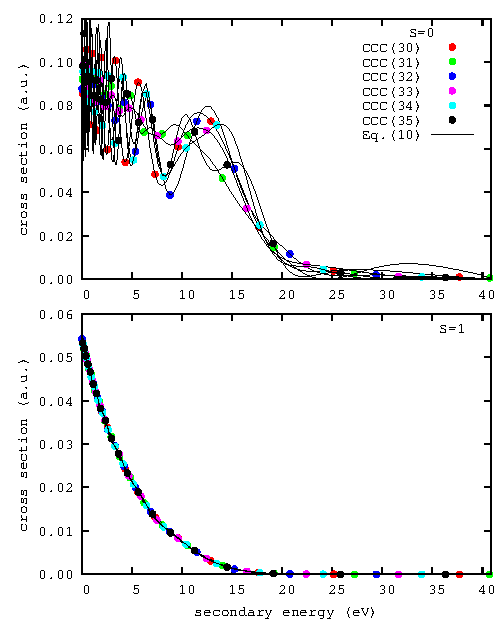
\includegraphics{S_sdcs.eps}}
  \caption[e-H Singlet and Triplet SDCS with Ansatz]{
    Triplet and singlet single-differential cross sections (SDCS) for
    \SI{54.4}{\eV} electron-impact ionisation of hydrogen in S-wave model.
    Original figure from \cite[FIG 1]{PhysRevA.90.022710}.
  }
  \label{fig:physreva-90-022710-sdcs-s-wave}
\end{figure}

The behaviour of the ansatz in the vicinity of the equal-energy-sharing point
for the singlet case raised suspicions on the correctness of the ansatz.
As Stelbovics demonstrated \cite{PhysRevLett.83.1570} for the singlet case in
the S-wave model, the ionisation amplitudes exhibit a step-like behaviour about
the equal-energy-sharing point, which results in tumultuous behaviour in the CCC
calculation as a consequence of the discontinuity.
Despite this, the ionisation amplitudes are still expected to converge to half
the step height, and thus the SDCS to a quarter of the step height, at the point
of equal-energy-sharing.
It is therefore notable that the SDCS resulting from the ansatz did not
demonstrate any convergence to the expected quarter-step-height value.
This characteristic (or lack thereof) of the ansatz was seen to suggest that it
does not have a justifiable physical origin, despite of its otherwise acceptable
level of agreement.

Overall, the ansatz was suggested to constitute a useful interpolation scheme
which could be used with an expectation of accuracy, provided that the target
pseudoenergies formed a sufficiently dense discretisation of the outgoing energy
continuum.
That the ansatz can be readily extended to more complex targets, eliminating the
need for the interpolation over ionisation amplitudes while retaining an
acceptable level of validity, is what motivates this project.

\clearpage

\subsection{Electron-Impact Helium Ionisation}
\label{sec:e-he-ionisation}

Having examined the CCC approach to electron-impact ionisation of hydrogen, the
simplest atomic target, we now consider its application to a helium target; this
forms the motivation for this project, as we consider the electron-impact
ionisation of helium, with and without excitation.

\subsubsection{Additional Considerations for a Helium Target}
\label{sec:e-he-target}

Much of the CCC method, derived in \autoref{sec:ccc-method}, is naturally
extended from a hydrogen target to a helium target.
However, the presence of an additional electron does introduce additional
complexity in the modelling of target structure, as target states are no longer
described in terms of a single wavefunction, but rather a slater determinant of
one-electron wavefunctions - significantly increasing the dimensionality of the
calculation.
Additionally, whereas singly-ionised hydrogen is left with no target structure,
singly-ionised helium retains an electron which may be left in an excited state
or the ground state - referred to as ionisation with, or without, excitation
respectively.
Helium also exhibits the phenomena of possessing doubly-excited states which are
autoionising, such as $2\mathrm{s}2\mathrm{s} {}^{1}\mathrm{S}$,
$2\mathrm{s}3\mathrm{s} {}^{1}\mathrm{S}$, and
$2\mathrm{s}3\mathrm{s} {}^{3}\mathrm{S}$ \cite{Plottke_2004}.
A feature of these states is that they are discrete states yet with positive
energy, and hence their calculation is dependent on an accurate description of
the helium target continuum by the target pseudostates.

Furthermore, the helium target states can have spin $S \in \lrset{0, 1}$,
which couples with the spin of the projectile electron $s_{0} = \tfrac{1}{2}$,
increasing the complexity of the spin algebra beyond that encountered for
hydrogen.
We have described the construction of Slater determinants and provided a brief
overview of how their dimensionality may be handled in
\autoref{sec:target-states}, however we shall not describe in explicit detail
here how they are constructed in the CCC method.
It suffices to say that the helium target structure is constructed using a
partially frozen-core model, with one electron state being expanded in only a
small number $n_{\rm{c}}$ of orbitals, while the other electron state is
expanded in a larger number.
This approach has been demonstrated to represent the target structure suitably
well for scattering calculations, however the number of core orbitals required
varies for different processes.
For a more detailed treatment of the target structure, and the handling of spin
in electron-impact helium collisions, we refer to the work of Fursa, Bray and
Stelbovics \cite{PhysRevA.52.1279, PhysRevLett.76.2674, Fursa_1997,
  PhysRevA.63.040702}.

Lastly, we note that the explicitly anti-symmetrised potential
\autoref{eq:ccc-v}, for a helium target, is of the form
\begin{equation}
  \label{eq:ccc-v-he}
  \hat{V}
  =
  \hat{V}_{0}
  +
  \hat{V}_{0, 1}
  +
  \hat{V}_{0, 2}
  -
  \hat{U}_{0}
  +
  \lrsq
  {
    E
    -
    \hat{H}
  }
  \lrsq
  {
    \hat{P}_{0, 1}
    +
    \hat{P}_{0, 2}
  }
  ,
\end{equation}
where it should be reiterated that this potential is modified form of the
asymptotic potential, and does not include the potential terms of the target
Hamiltonian.

\subsubsection{Convergent Close-Coupling Calculations}
\label{sec:e-he-ccc-calculations}

The CCC method, having been proven capable of modelling elastic scattering and
discrete excitations \cite{PhysRevA.46.6995} as well as ionisation processes
\cite{PhysRevLett.70.746, PhysRevLett.78.4721, PhysRevLett.83.1570} for
electron scattering on hydrogen, was extended to helium by Fursa and Bray
\cite{PhysRevA.52.1279, PhysRevLett.76.2674, Fursa_1997}.

It was demonstrated by Fursa and Bray \cite{Fursa_1997} that the CCC method
yielded accurate cross sections for elastic scattering and discrete excitations
of the ground state of helium, $2{}^{1}\mathrm{S}$, with a frozen core model
$n_{\rm{c}} = 1$.
However, it was observed that the cross sections for the metastable state
$2{}^{3}\mathrm{S}$ did not produce acceptable agreement with experimental
values and other computational values found in the literature.
A later investigation by Bray and Fursa \cite{PhysRevA.63.040702}, incorporating
the insights gained from the analysis of electron-impact ionisation of hydrogen,
suggested that the CCC method yielded accurate ionisation amplitudes and
differential cross sections for electron-impact ionisation of helium without
excitation.
Further investigation by Plottke \textit{et al.} \cite{Plottke_2004} into
electron-impact excitation of helium indicated that the convergence of the
autoionising doubly-excited discrete states was more involved than for the
singly-excited bound states.
However, convergence was demonstrated for these autoionising states.

Notably, the Exterior Complex Scaling (ECS) method was applied by Bartlett and
Stelbovics \cite{PhysRevA.81.022715, PhysRevA.81.022716}, in the context of the
S-wave model, to yield comprehensive total and differential cross sections for
double ionisation, ionisation with excitation, and double excitation for helium.
Agreement between the ECS and CCC methods was found for the total ionisation
cross section without excitation, but not with excitation.
Furthermore, an acceptable level of agreement between the methods was not found
for the double excitation cross sections.

In summary, the CCC method is demonstrated to suitably model electron-impact
collisions with helium in the ground state $2{}^{1}\mathrm{S}$, including
elastic scattering, single-excitation and single-ionisation scattering
processes.
However, further development is required to calculate double excitation cross
sections which are in agreement with ECS calculations, and to calculate cross
sections which are in agreement with experimental values for the metastable
state $2{}^{3}\mathrm{S}$ of helium.

\section{Conclusion}
\label{sec:conclusion}

We have reviewed the development of the treatment of ionisation in the CCC
method, within the context of the S-wave model, and seen that it does indeed
yield accuracte calculations for the ionisation amplitudes and differential
cross sections for electron-impact ionisation of hydrogen.
The manifestation of a Fourier-like expansion of a step-like term in the SDCS of
hydrogen was demonstrated to occur in CCC calculations, and was shown to be
expected on theoretical grounds \cite{PhysRevLett.78.4721, PhysRevLett.83.1570}.
Implementing an appropriate treatment for the resulting irregular behaviour of
the SDCS was then demonstrated to yield calculations which were in remarkable
agreement with those from experimental data as well as from other computational
techniques \cite{PhysRevLett.89.273201}.

The ansatz of Zatsarinny and Bartschat \cite{PhysRevLett.107.023203} was
determined to be non-physical, and yet still capable of functioning as an
effective interpolation scheme which circumvents the restriction to evaluating
the ionisation amplitudes only at a countable number of outgoing projectile
energies \cite{PhysRevA.90.022710}.

Finally, the CCC approach to electron-impact collisions on helium, in the ground
state $2{}^{1}\mathrm{S}$, was shown to be in agreement with experiment and
other computational methods.
What remains, for this project, is to investigate the applicability of the
ansatz of Zatsarinny and Bartschat to electron-impact ionisation of helium, and
to examine under what conditions the ansatz is most and least effective, in a
similar manner as done by Bray \textit{et al.} \cite{PhysRevA.90.022710}.
If the suitability of ansatz is established for single-ionisation without
excitation, then it shall be examined further for the case of ionisation with
excitation.

\clearpage

\bibliography{references}

\clearpage

% \appendix

% \section{Properties of Utilised Bases}
% \label{app:properties}

% \subsection{Spherical Harmonics}
% \label{app:spherical-harmonics}

% \subsubsection{Completeness}
% \label{app:spherical-harmonic-completeness}

% \todo[spherical harmonic completeness]{
%   Prove that the set of spherical harmonics forms,
%   $\lrset{Y_{l}^{-l}\lr{\Omega}, \dotsc, Y_{l}^{l}\lr{\Omega}}_{l = 0}^{\infty}$,
%   forms an orthonormal, complete basis for the Hilbert space
%   $L^{2}\lr{S^{2}}$.
% }

% \subsection{Laguerre Radial Basis}
% \label{app:laguerre-radial-basis}

% \subsubsection{Completeness}
% \label{app:laguerre-radial-completeness}

% \todo[laguerre radial completeness]{
%   Prove that the Laguerre radial basis functions,
%   $\lrset{\xi_{k, l}\lr{r}}_{k = 1}^{\infty}$, for each $l$, forms a complete
%   basis for the Hilbert space $L^{2}\lr{[0, \infty)}$.
% }

% \subsection{Laguerre Basis}
% \label{app:laguerre-basis}

% \subsubsection{Completeness}
% \label{app:laguerre-completeness}

% It is shown in \autoref{app:laguerre-radial-completeness}, that the Laguerre
% radial basis functions, $\lrset{\xi_{k, l}\lr{r}}_{k = 1}^{\infty}$, for each
% $l$, forms a complete basis for the Hilbert space $L^{2}\lr{[0, \infty)}$.
% Similarly, it is also shown in \autoref{app:spherical-harmonic-completeness},
% that the set of spherical harmonics,
% $\lrset{Y_{l}^{-l}\lr{\Omega}, \dotsc, Y_{l}^{l}\lr{\Omega}}_{l = 0}^{\infty}$,
% forms an orthonormal, complete basis for the Hilbert space $L^{2}\lr{S^{2}}$.
% Hence, the Laguerre basis functions
% $\lrset{\varphi_{i}\lr{r, \Omega}}_{i = 1}^{\infty}$, form a complete basis
% for the Hilbert space $L^{2}\lr{\real^{3}}$.

% \subsection{Plane Waves}
% \label{app:plane-waves}

% \section{Numerical Techniques}
% \label{app:numerical-techniques}

% \subsection{Basis Expansion}
% \label{app:basis-expansion}

% \todo[basis expansion]{
%   Elaborate on the method of basis expansion for Hilbert spaces.
% }

% \subsection{Diagonalisation}
% \label{app:diagonalisation}

% \todo[target diagonalisation]{
%   Elaborate on the diagonalisation procedure for the target states.
% }

% \clearpage

\todos

\end{document}